\documentclass[a4paper,11pt,titlepage,uplatex]{jsarticle}

% プリアンブルを外部ファイル化しておきました。中身はmacro.texで確認できます。

\usepackage[dvipdfmx]{graphicx,xcolor}% ドライバ指定
\usepackage[top=30truemm,bottom=30truemm,left=25truemm,right=25truemm]{geometry} % 余白設定

% 画像
\usepackage{here, subfig}
\usepackage{docmute} % ファイル分割用
\usepackage[cc]{titlepic}

% 数式関連
\usepackage{amsmath,amsfonts,amssymb,mathtools,amsthm}
\usepackage{bm} % ボールド体のベクトルを出力するときには\vb{a}ではなく\bm{a}としてください。\bmの方が綺麗に出力できる。
\usepackage{empheq} % 連立方程式をきれいに書いてくれる
\usepackage{physics} % 微分記号とか
\usepackage[separate-uncertainty]{siunitx} % SIUNITX

% 数式、図、表番号の変更
\makeatletter
\@addtoreset{equation}{section} % 章ごとに番号をリセット
\@addtoreset{figure}{section}
\@addtoreset{table}{section}
\def\theequation{\thesection.\arabic{equation}} % 章.何番目 と変更
\def\thefigure{\thesection.\arabic{figure}}
\def\thetable{\thesection.\arabic{table}}
\makeatother

% -------------------
% 定理環境付近
\usepackage{tcolorbox} % 色付きの囲み
\tcbuselibrary{breakable, skins, theorems}
\usepackage{ascmac} % 囲み \begin{itembox}ができる。

% ----------

\usepackage{enumitem} % enumium環境いじるために必要
\renewcommand{\labelenumi}{\theenumi.}
\renewcommand{\theenumi}{\Alph{enumi}}

% ------------ url関係
\usepackage{url}
\usepackage[dvipdfmx]{hyperref}
\hypersetup{
	 colorlinks=true,
	 citecolor=blue,
	 linkcolor=black,
	 urlcolor=blue
}
\usepackage{pxjahyper}
% ---------

% 表関連のパッケージ
\usepackage{booktabs}
\usepackage{multirow}
\usepackage{longtable}
\usepackage{arydshln}% 表で破線を使うため
\usepackage{multicol}
% longtableをusepackageする場合は順番が重要らしいです。longtableとarydshlnの順番逆にしたらエラーはく(コンパイルはできるが…)

\renewcommand{\labelitemii}{・}

\usepackage[greek, japanese]{babel}
\usepackage{teubner}	% 古代(古典)ギリシア語表記指定



% 大槻使用
\usepackage{color}
\newcommand{\red}[1]{\textcolor{red}{#1}}
\newcommand{\blue}[1]{\textcolor{blue}{#1}}
\usepackage{ulem}

% 能崎使用
%背景
\usepackage{wallpaper}

\begin{document}

% \tableofcontents % 目次を作成
\newpage
\section{構造系}

\blue{青文字は部内用のみ記載事項}\footnote{\red{赤文字はメモ用。最終的に消える予定}}

\subsection{機体概要}
機体諸元を表\ref{s_59syogen}に示す。
また、機体外形図、各部材位置、各部品詳細をそれぞれ図\ref{s_gaikei}、図\ref{s_iti}、表\ref{s_buhin}に示す。
また、実機写真を図\ref{s_real1}、図\ref{s_real2}に示す。

\begin{table}[H]
    \centering
    \caption{機体諸元}
    \begin{tabular}{ccl} \toprule
        名称 & 諸元 & 備考\\\midrule
        機体名称 & IRIS(C-59J)\\
        全長 & \SI{1541}{mm} & ピトー管あり\\
         & \SI{1486}{mm} & ピトー管なし\\
        直径 & \SI{91}{mm}\\
        乾燥質量 & \SI{5944}{g}\\
        重心位置 & \SI{707}{mm} & 機体後端より\\
        圧力中心位置 & \SI{523}{mm} & 機体後端より\\
        静安定静余裕 & 11.6 & 最小値\\
         & 12.8 & 最大値\\
        \bottomrule
    \end{tabular}
    \label{s_59syogen}
\end{table}

\begin{figure}[H]
    \centering
    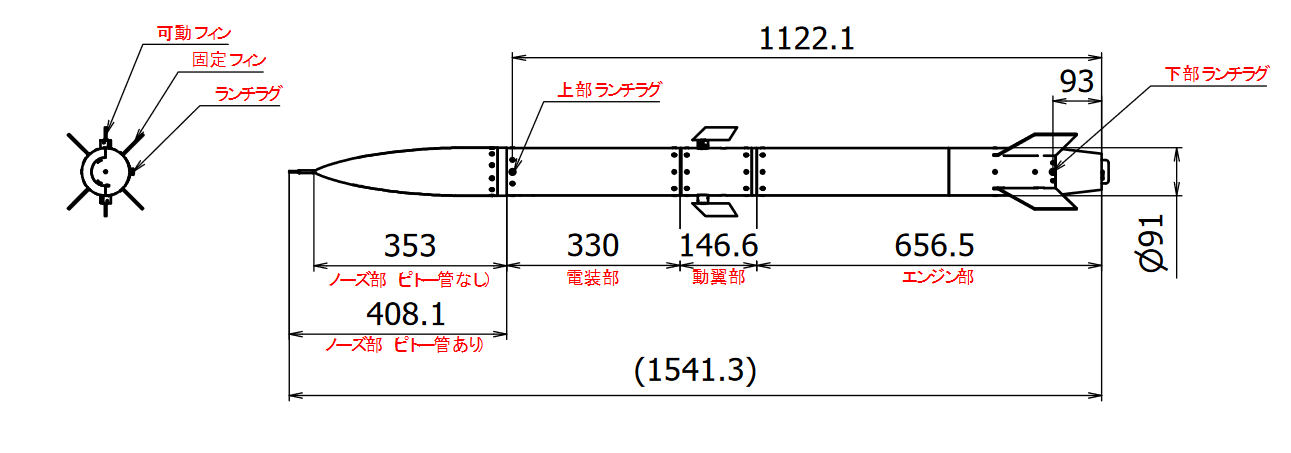
\includegraphics[scale = 0.6]{pic_str/s_sunpou.png}
    \caption{機体外形図}
    \label{s_gaikei}
\end{figure}

\begin{figure}[H]
    \centering
    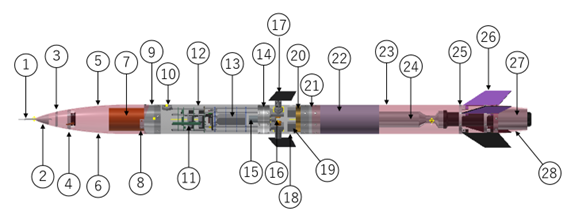
\includegraphics{pic_str/s_iti.png}
    \caption{各部材位置}
    \label{s_iti}
\end{figure} 

\renewcommand{\arraystretch}{0.9}
\begin{longtable}[H]{cclll} 
    \caption{各部品詳細図}
    \label{s_buhin}\\
        \toprule
        区画&No.&部品名&材質&型番及び説明\\ \hline \endhead
        ノーズ部&1&ピトー管&A5052&内製、\ref{pito}項に記載\\
         &2&ノーズトップ&ABS&ピトー管固定用\\
         &3&ピトー管用基板&N/A&電装概要に記載\\
         &4&減速機構&N/A&従来機体から踏襲\\
         &5&ノーズコーン&CFRP&\\
         &6&フェアリング&CFRP&開放部\\
         &7&パラシュート&ナイロン&\\
         &8&リカバリーネイル&ABS&フェアリング抑え\\\midrule
         &9&NAカプラー&A5052&\\ \midrule
        電装部&10&電源投入スイッチ&ABS&\ref{switch}項に記載\\
         &11&電装タワー&N/A&\ref{avi_all}章に記載\\
         &12&電装チューブ&GFRP&\\
         &13&LiFeバッテリー&N/A&ROBOパワーセル F3-1450タイプ(Li-Fe)\\ \midrule
         &14&ARカプラー&A5052&\\ \midrule
        動翼部&15&動翼制御用モータ&N/A&Maxon(製品番号:134164、110160、201937)\\
         &16&動翼機構&N/A&\ref{douyoku}節に記載\\
         &17&可動フィン&アクリル&\\
         &18&動翼チューブ&CFRP\\
         &19&カメラ&N/A&MD25\\
         &20&錘&真鍮&\\\midrule     
         &21&REカプラー&A5052&\\ \midrule
        エンジン部&22&スタイロフォーム&N/A&エンジン抑え\\
         &23&エンジンチューブ&CFRP\\
         &24&エンジン&N/A&HyperTEK J250\\
         &25&フィンブロック&ABS&フィン固定用\\
         &26&固定フィン&アクリル&\\
         &27&エンジン受け&A5052&2部品で構成\\
         &28&テールコーン&ABS&\ref{tale}項に記載\\ 
         \bottomrule
\end{longtable}
\renewcommand{\arraystretch}{1.0}

 
\begin{figure}[H]
    \centering
    \includegraphics[scale = 0.1]{pic_str/s_59_real_pic.jpg}
    \caption{実機写真} 
    \label{s_real1}
\end{figure}

\begin{figure}[H]
    \centering
    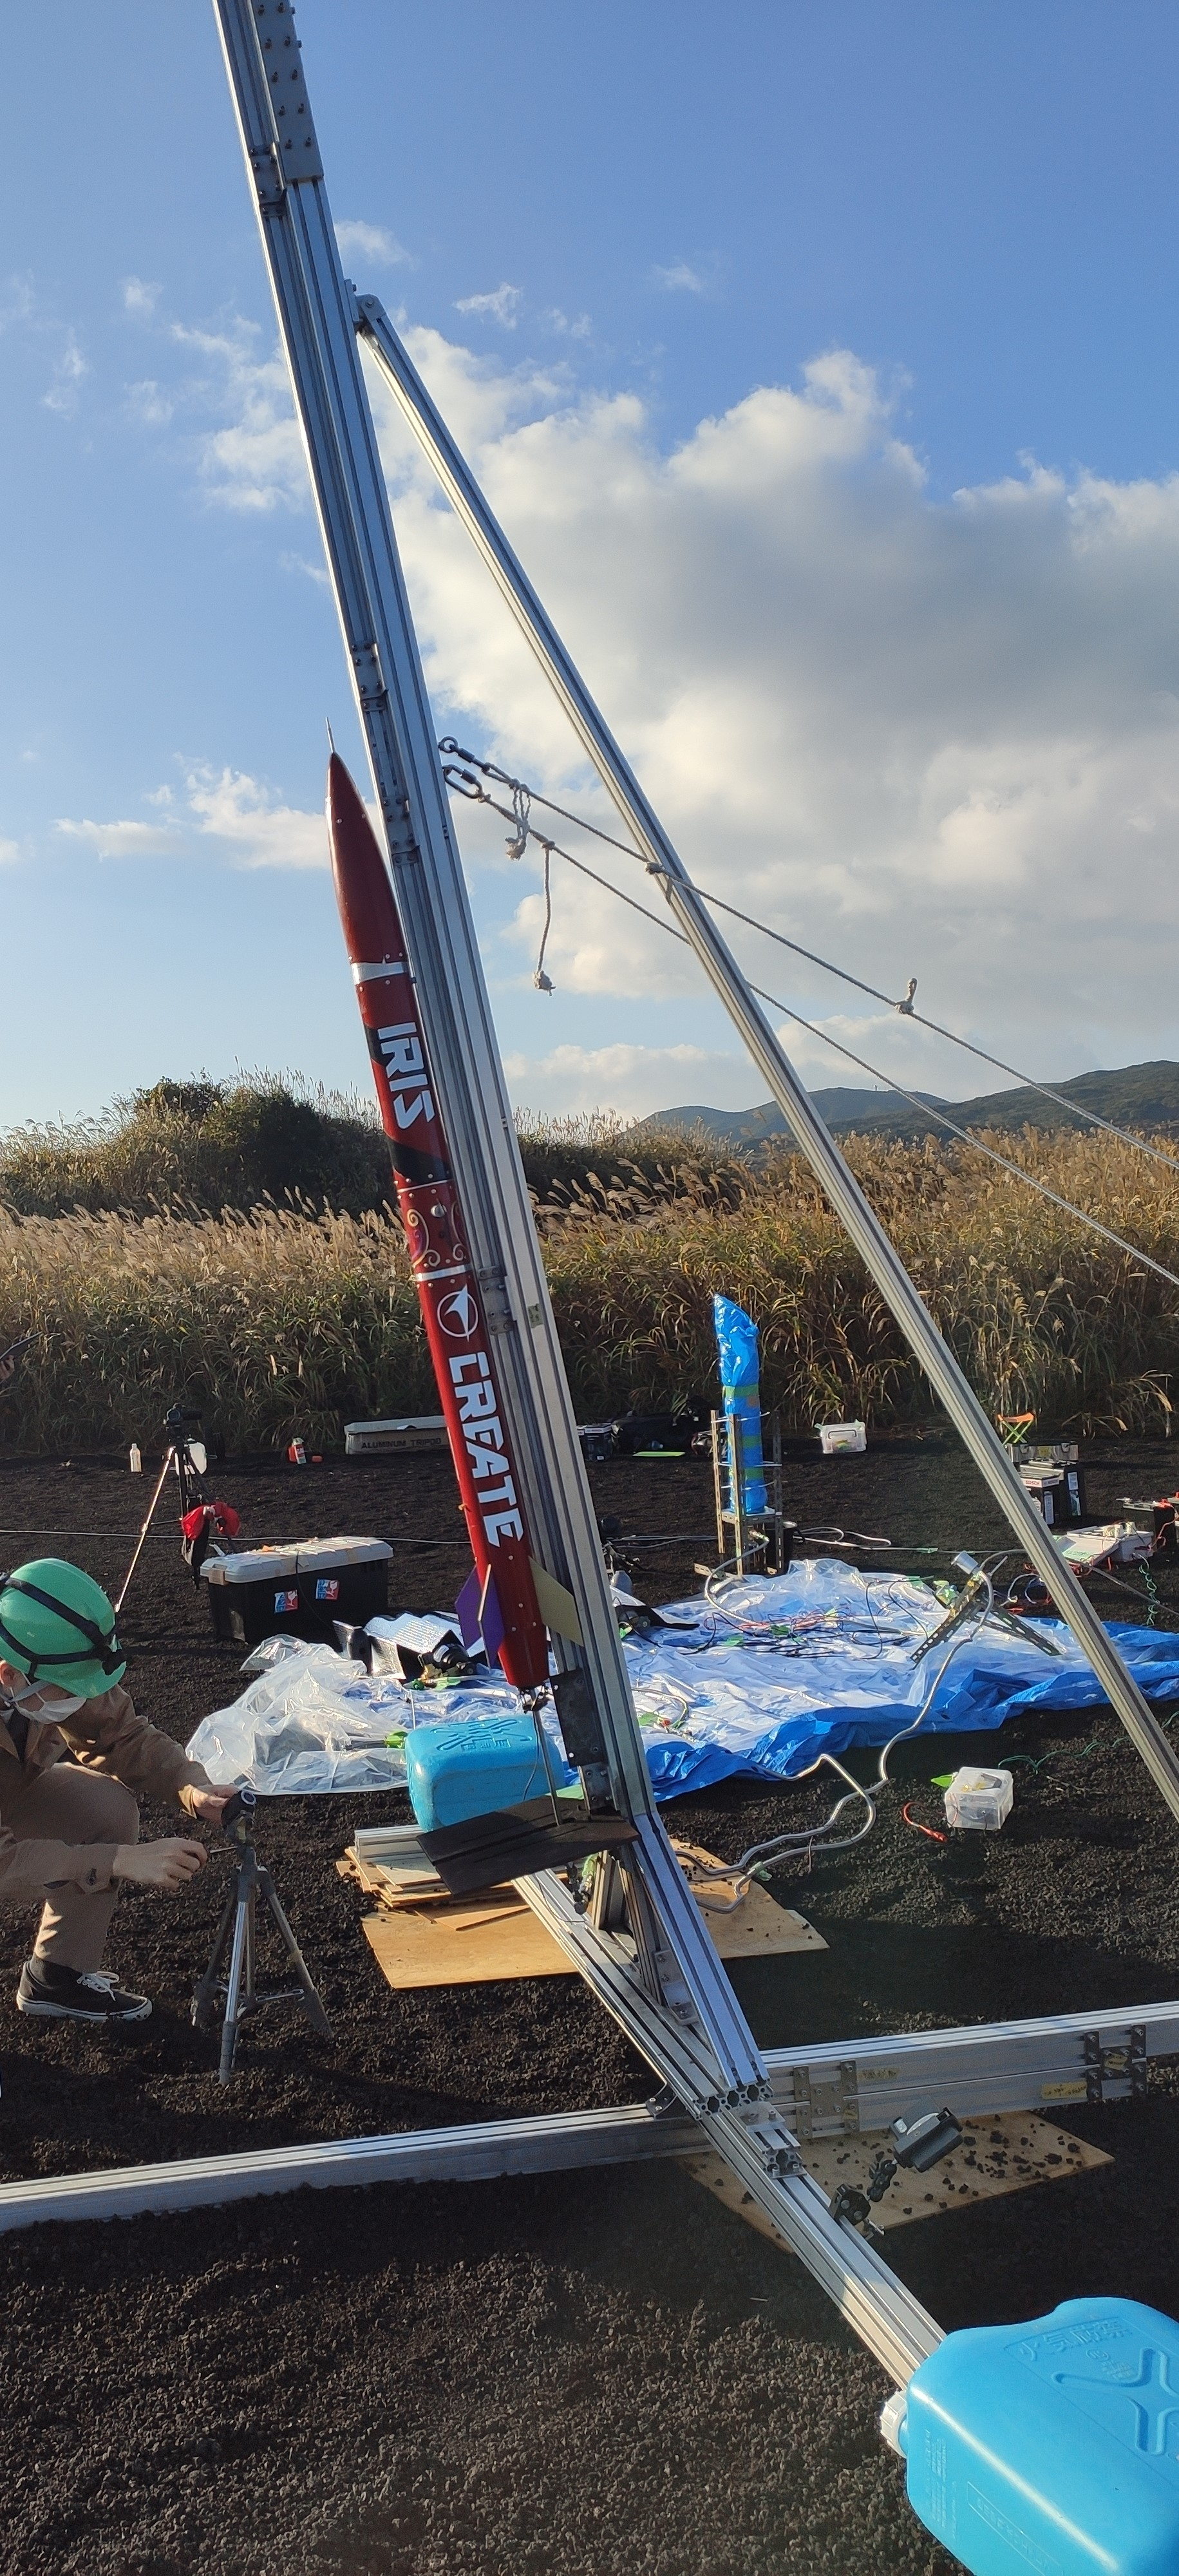
\includegraphics[scale = 0.1]{pic_str/s_59_launcher.jpg}
    \caption{実機写真(ランチャー挿入)}
    \label{s_real2}
\end{figure}

本機は従来のCREATE機体をベースに設計しており、ロール制御ミッション達成のため新たに可動フィンを設置している。
図\ref{s_gaikei}左側記載の側面図に示すように、固定フィン4枚、可動フィン2枚を搭載している。
フィンの位相角は、ランチラグ\SI{0}{deg}としたとき、固定用フィンは\SI{45}{deg}、\SI{135}{deg}、\SI{225}{deg}、\SI{315}{deg}であり、可動フィンは\SI{90}{deg}、\SI{270}{deg}となっている。
これは、可動フィンによって発生した乱流が後方のフィンに影響を与えないようにするためである。
また、可動フィンを取り付けない状態と取り付けた状態の両方で$F_{ST}$の基準を満たしていることをシミュレーションで確認しており、空力安定性は保たれている。

\subsection{動翼機構}
\label{douyoku}

\subsubsection{動翼機構概要}本節では、ロール制御ミッションのために新たに追加した動翼部について記す。
動翼機構のcad図と写真、外形の様子をそれぞれ図\ref{s_r_all}、図\ref{s_r_pic}、図\ref{s_r_outer}に示す。

\begin{figure}[H]
    \centering
    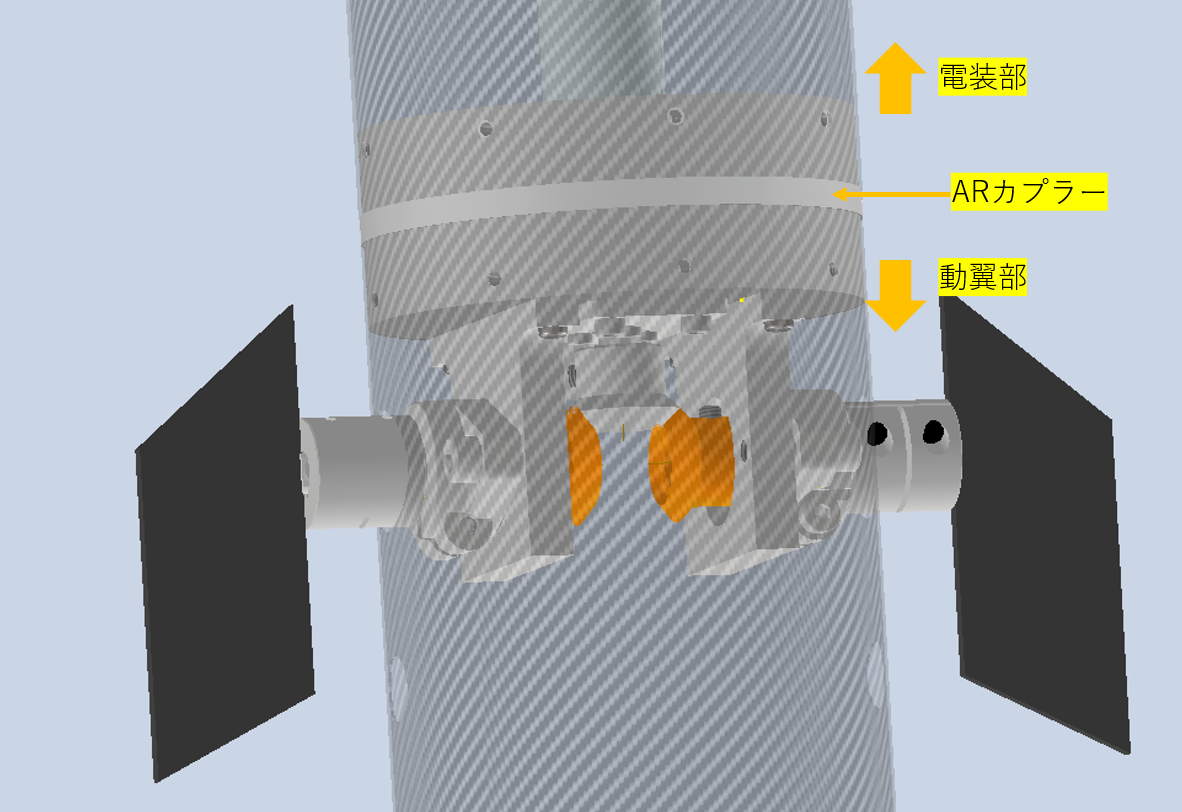
\includegraphics[scale = 0.3]{pic_str/s_roll_all.png}
    \caption{動翼機構cad図}
    \label{s_r_all}
\end{figure}

\begin{figure}[H]
    \centering
    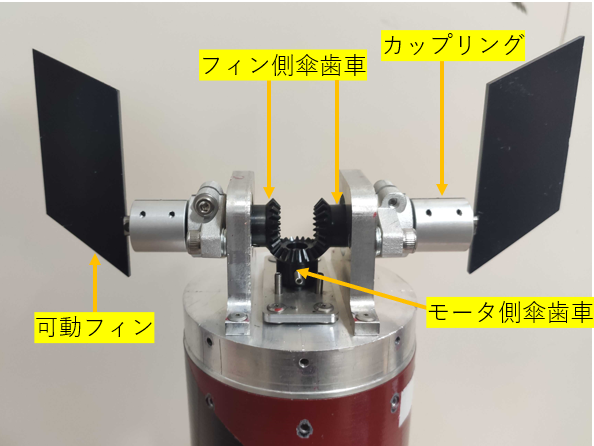
\includegraphics[scale = 0.6]{pic_str/s_r_pic.png}
    \caption{動翼機構}
    \label{s_r_pic}
\end{figure}

\begin{figure}[H]
    \centering
    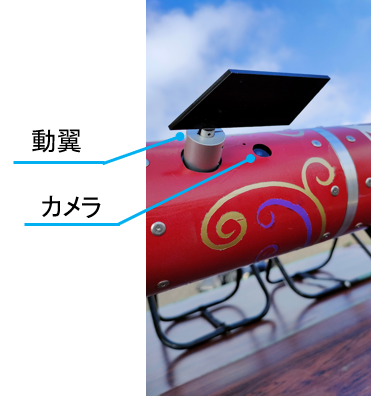
\includegraphics[scale = 0.55]{pic_str/s_r_outer.png}
    \caption{動翼付近外形}
    \label{s_r_outer}
\end{figure}

傘歯車を介して、モータの回転量を左右2枚の可動フィンに伝える機構になっている。
この機構にすることで、2枚の可動フィンが連動し、かつ同じ量だけ回転するようになっている\footnote{
傘歯車を使用せず、左右にサーボモータを設置しフィンを回転させる方法も検討したが、高精度の制御ができるモータを使用したい、左右2つのフィン回転量が等しいことを担保したい、という2点よりこの機構を採用した。
代わりに傘歯車のバックラッシが小さく、かつ摩擦補償が小さい機構の製作が必要となった。}

\subsubsection{\blue{動翼機構詳細}}
動翼機構は,図\ref{s_r_pic}に示すように、モーターモジュールと可動フィンモジュールに分かれている。
図\ref{s_r_motorCAD}、\ref{s_r_finCAD}にモーターモジュール、可動フィンモジュールの構成図を示す.また,表\ref{s_r_table}に主な構成部品表を示す.
ただし、図ではパーツ間の接触を可視化すべく一部パーツに色を付けているが、実際は塗装されていない。

\begin{figure}[H]
    \centering
    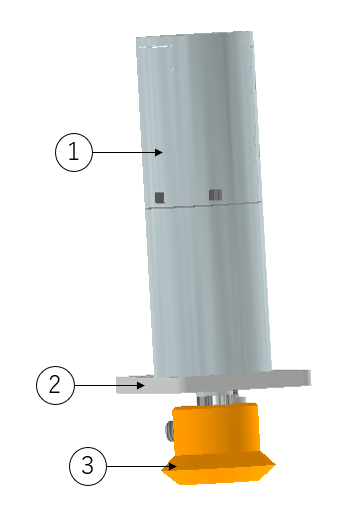
\includegraphics[scale = 0.5]{pic_str/s_r_motorCAD.png}
    \caption{モーターモジュール構成図}
    \label{s_r_motorCAD}
\end{figure}

\begin{figure}[H]
    \centering
    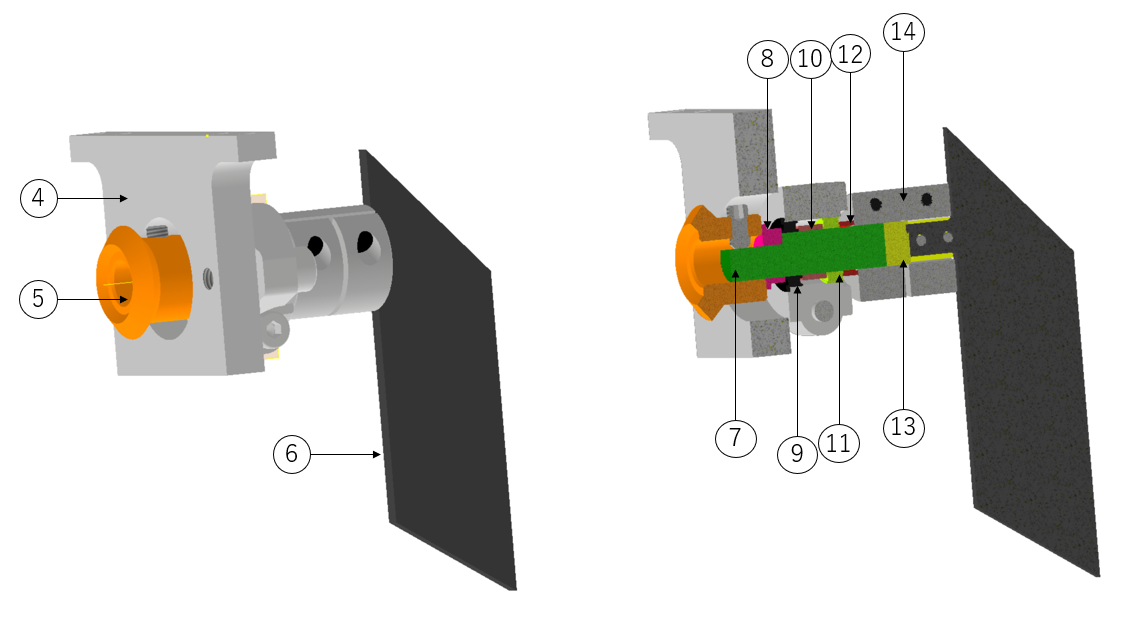
\includegraphics[scale = 0.5]{pic_str/s_r_finCAD.png}
    \caption{可動フィンモジュール構成図とその断面図}
    \label{s_r_finCAD}
\end{figure}

\begin{table}[H]
    \centering
    \caption{動翼機構構成部品}
    \begin{tabular}{cllp{70mm}}\toprule
         No.&部品名&型番&材質、備考\\ \midrule
         1&モータ&表\ref{s_buhin}(No.15)参照&ARカプラーを貫通させ、モータのコネクタを電装部側になるように配置。\\
         2&モーター固定用板&内製&A5052製。ARカプラーとモーターの固定用。図面を以下の図\red{1}に示す。\\
         3&モータ側傘歯車&KGEASTB-1.0-2020-8&モーターとはイモネジ(型番:MSSFS3-12)で固定している。その際カラー(型番:PSCCN4-8b)を挟んだ。\\ \midrule
         4&固定用板&内製&A5052製。ARカプラーと\ \ の固定用。図面を以下の図\red{2}に示す。\\
         5&フィン側傘歯車&KGEASTB-1.0-2020-8&回転軸とイモネジ(型番:MSSFS4-8)で固定している。\\
         6&可動フィン&内製&アクリル製。\ \ と超極ネジ(型番:CBSTNR2-6)図面を\red{3}に示す。\\
         7&回転軸&内製&SUS304製。図面を\red{4}に示す。\\
         8&歯車位置調整ジグ&内製&A5052製。図面を\red{5}に示す。\\
         9&フランジ付きベアリング&FL678ZZ&固定用板をフランジにあて位置。\\
         10&ベアリング間位置調整ジグ&内製&\\
         11&ベアリング&SUTB128A5ZZ&\\
         12&カップリング位置調整ジグ&WSSB10-8-3&\\
         13&フィン固定軸&内製&SUS304製。図面を\red{6}に示す。\\
         14&カップリング&CPRC20-8-8&フィン位相調節用\\ \bottomrule
    \end{tabular}
    \label{s_r_table}
\end{table}


以下に特記点を示す。
\begin{itemize}
    \item フィン側傘歯車と可動フィンは連動して回転するようになっているが、左右2枚の可動フィンの位相を合わすために、カップリングを設置している。
    現地組立では水準器を使用し、2枚の可動フィンと機軸の水平度を測ることでフィン位相を合わせた。
    \\
    \item 電装計器の誤作動、電源喪失、ピトー管の値異常などが原因で可動フィンが想定より多く回転してしまい、機体の姿勢が不安定になることを防ぐため、フィンの回転制御角を物理的に制限する機構を搭載している。この機構のCAD図を図\ref{s_r_kadouiki}に示す。
    \begin{figure}[H]
        \centering
        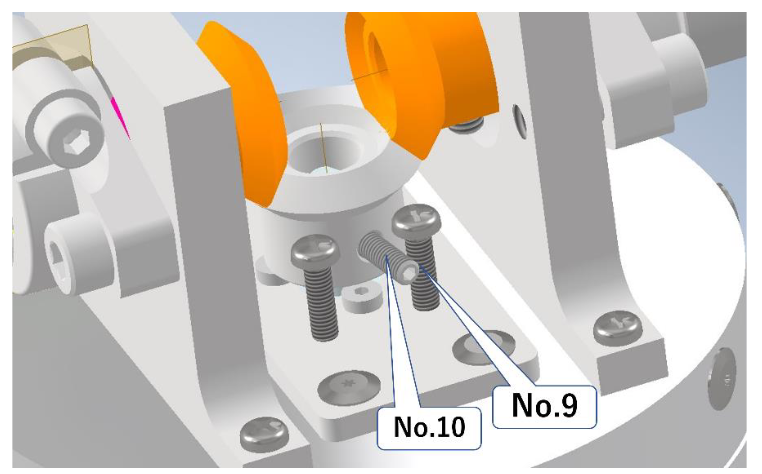
\includegraphics[scale = 0.5]{pic_str/s_r_kadouiki.png}
        \caption{回転角制御機構}
        \label{s_r_kadouiki}
    \end{figure}
    モータと傘歯車を締結しているイモネジ(No.10)を仕様より長いものを使用し、回転角が中央\footnote{2つ設置してあるネジ(No.9)から等距離の地点。}から$\pm \SI{15}{deg}$ を超えるとネジ(No.9)にあたり、止まるようになっている。
    また、制御開始時にイモネジが中央に位置していないといけないが、カップリングの印をつけることで、フィン位相をあわせる際にイモネジが中央位置が分かるようにした。
    また、イモネジの正しい使い方をしていないため、通常使用時から緩むようになっていたが、ネジロックを使用することで緩まないようにした。
    \\
    \item 前述の通り、バックラッシを調整できるような設計を行った。主に加工誤差が原因で、傘歯車を設計値通りの場所に設置することができないため、製作後に傘歯車の位置をワッシャーとシムリングを挟むことでで調整できるようにした。
    具体的にはARカプラーとモーター固定用板、固定用板と\red{aaaa}の間にワッシャーやシムリングを挟んだ。
    \SI{0.1}{mm}ごとに傘歯車の位置を調整していき、バックラッシが小さくなり、かつ摩擦補償が小さくなる位置を決定した。
    \\
    \item 図\ref{s_r_outer}に示すように、動翼のすぐ下にカメラを設置した。これは飛行中に動翼が正常に動作していることを確認するため、及びロールしない映像を撮影するためである。
\end{itemize}


\subsubsection{改良点}
\red{位置決めピン。レーザーの位相合わせ。フィンの強度}

\subsection{従来機体からの変更点}

\subsubsection{ランチラグ}
ランチラグの規定があったため、ランチラグの仕様を変更した。
今回使用したランチラグの構成図及び図面を図\ref{s_launchlag}に、ランチラグの諸元を表\ref{s_launchlag_syo}に示す。
実際のランチラグの写真を図\ref{s_lan_pic}に示す。

\begin{figure}[H]
    \centering
    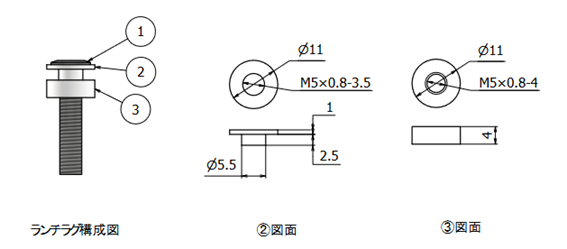
\includegraphics{pic_str/s_launchlag.png}
    \caption{ランチラグの構成図及び図面}
    \label{s_launchlag}
\end{figure}

\begin{table}[H]
    \centering
    \caption{ランチラグ諸元}
    \begin{tabular}{cccc}\toprule
         No.&部品名&材質&型番\\ \midrule
         1&M5超極低頭ボルト&SUS304& CSXSLH-SUS-M5-20\\
         2&樹脂ワッシャ(つば付きタイプ)&POM&FWHJ-D5.5-H1.1-V2.6-T1-L3.5\\
         3&樹脂ワッシャ&POM&FWSJJ-D11-V2.6-T4\\ \bottomrule
    \end{tabular}
    \label{s_launchlag_syo}
\end{table}

\begin{figure}[H]
    \centering
    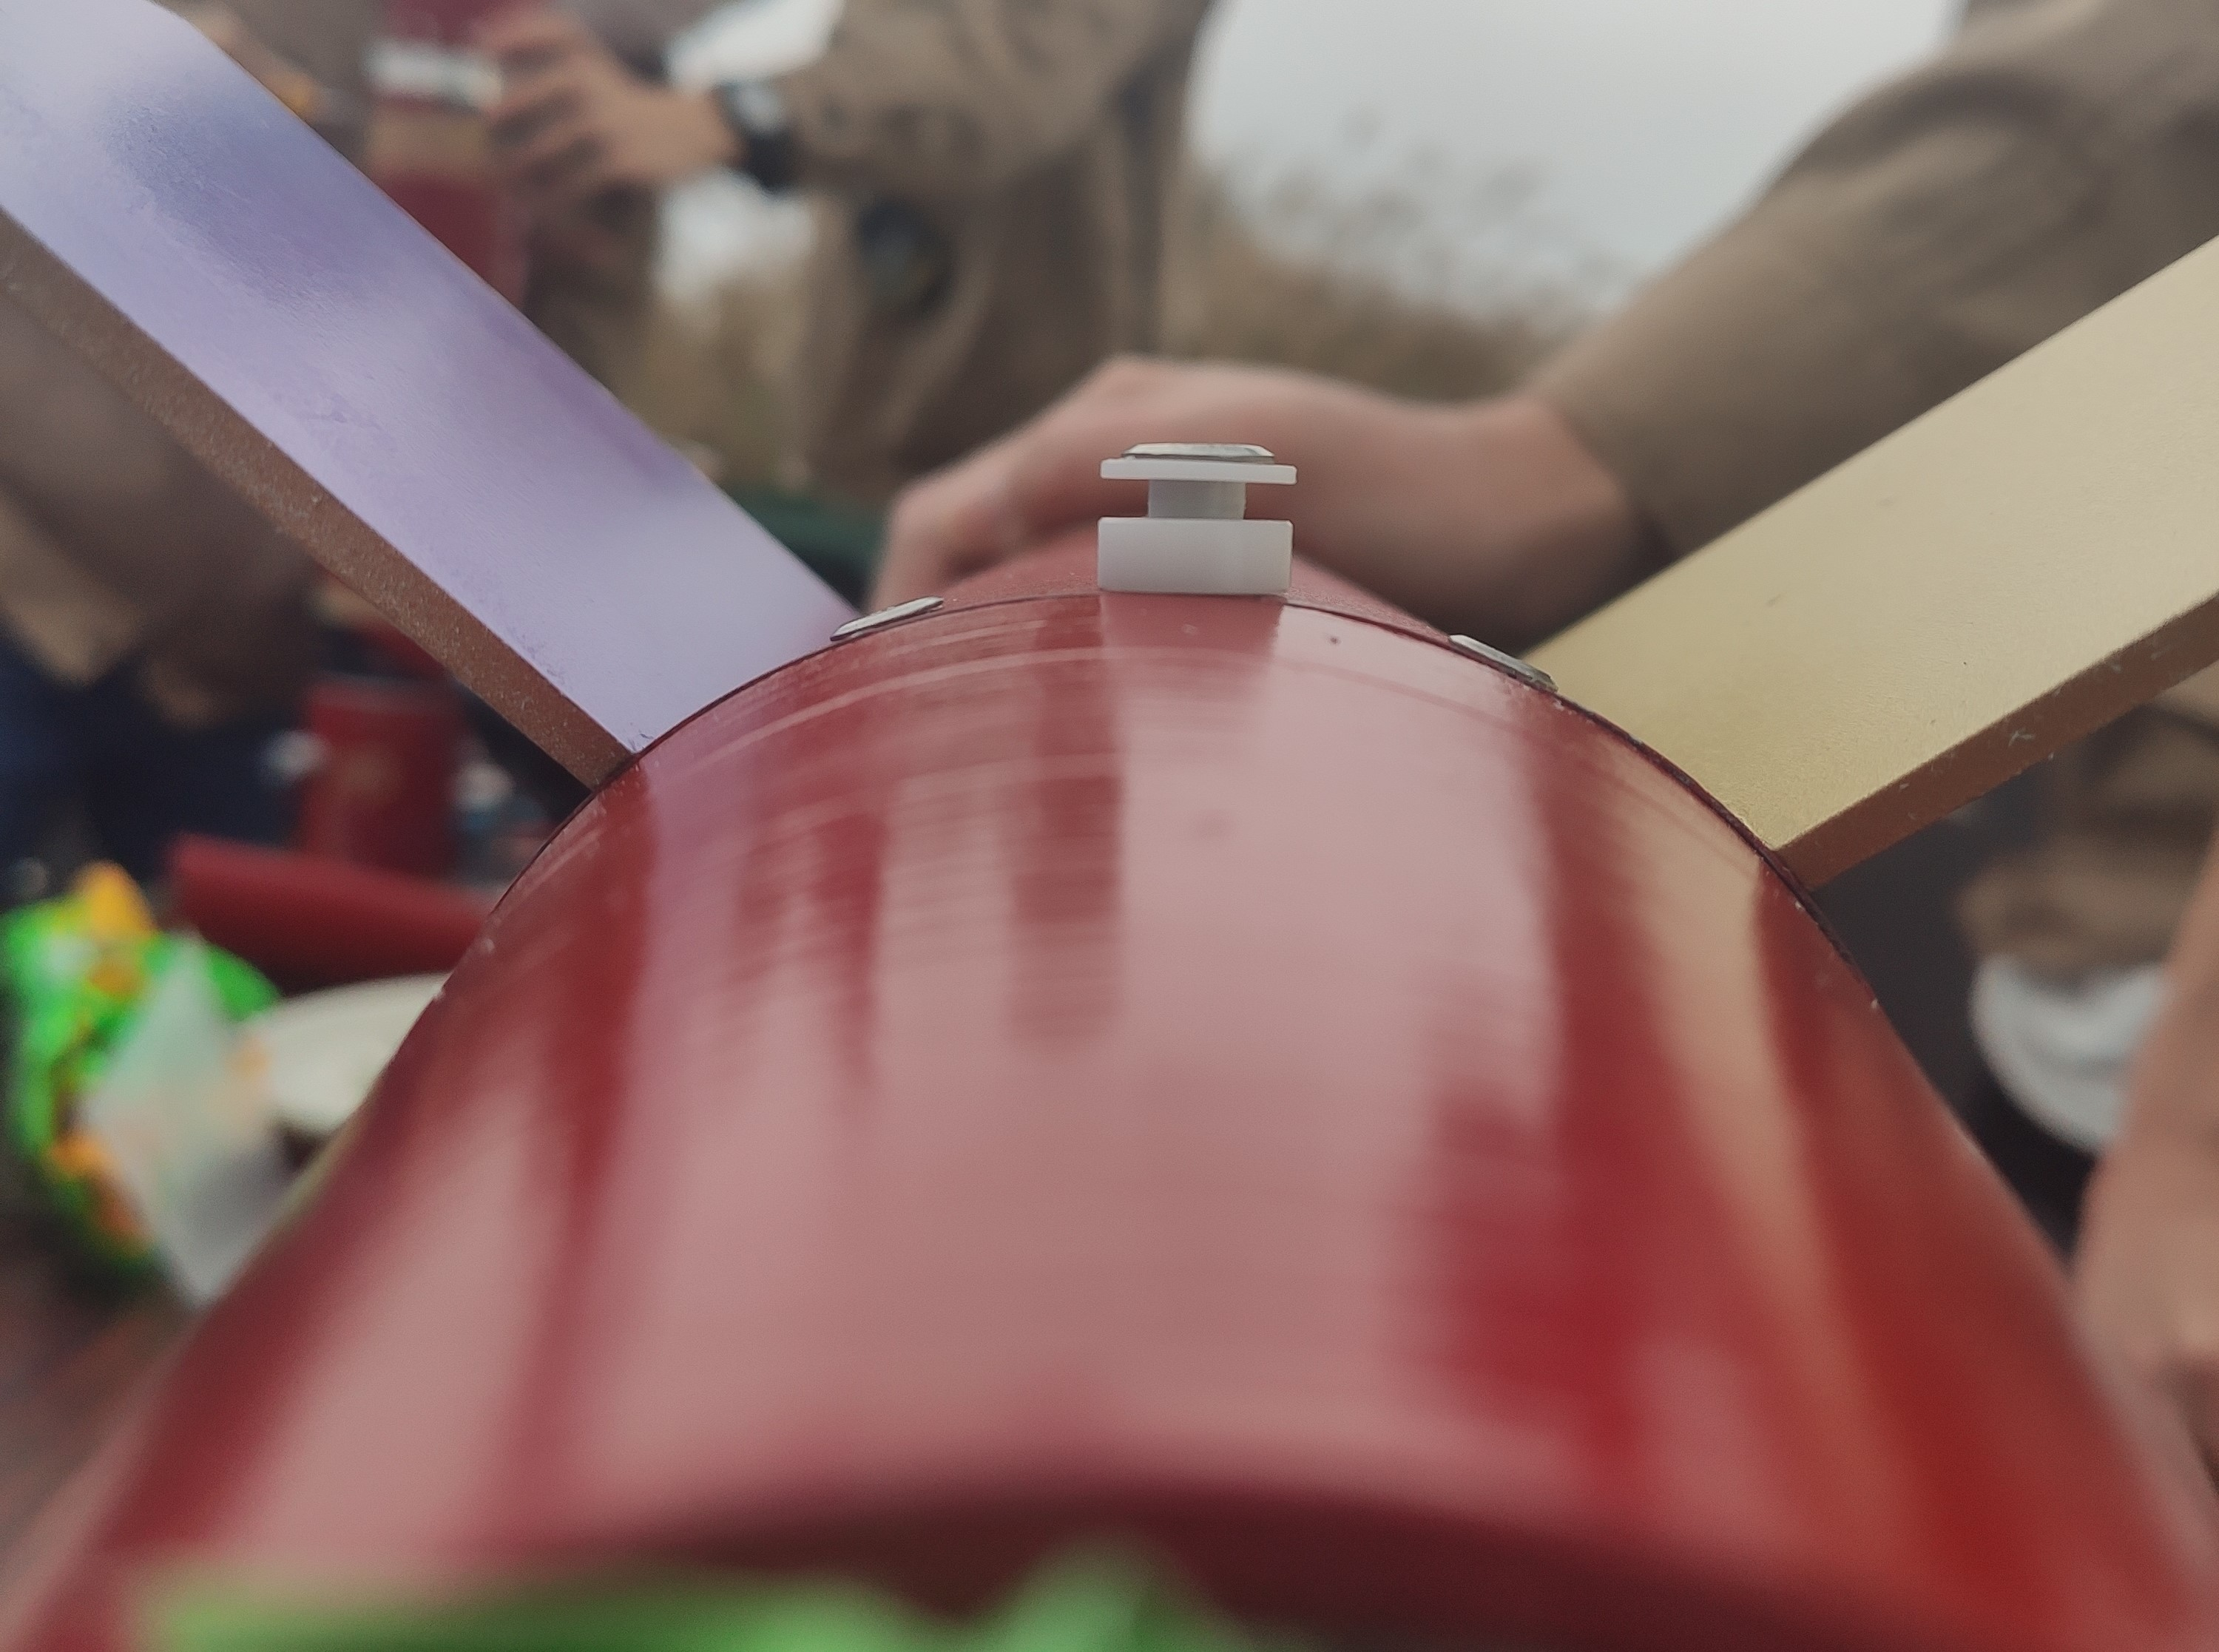
\includegraphics[scale = 0.1]{pic_str/s_lanch_pic.jpg}
    \caption{ランチラグ写真}
    \label{s_lan_pic}
\end{figure}

\red{ねじきり?}

また、ランチラグの締め付けトルクを決定する試験を行った。

\red{試験結果追記}


\subsubsection{ピトー管}
\label{pito}



\subsubsection{テールコーン}
\label{tale}

\red{ロケットの乱流を~~}のため、機体後端にテールコーンを設置した。
テールコーン付近の断面図を図\ref{s_tale_num}に、主な構成部品を表\ref{s_tale_table}に示す。
また、テールコーンの図面を図\ref{s_tale_zumen}に示す。

\begin{figure}[H]
    \centering
    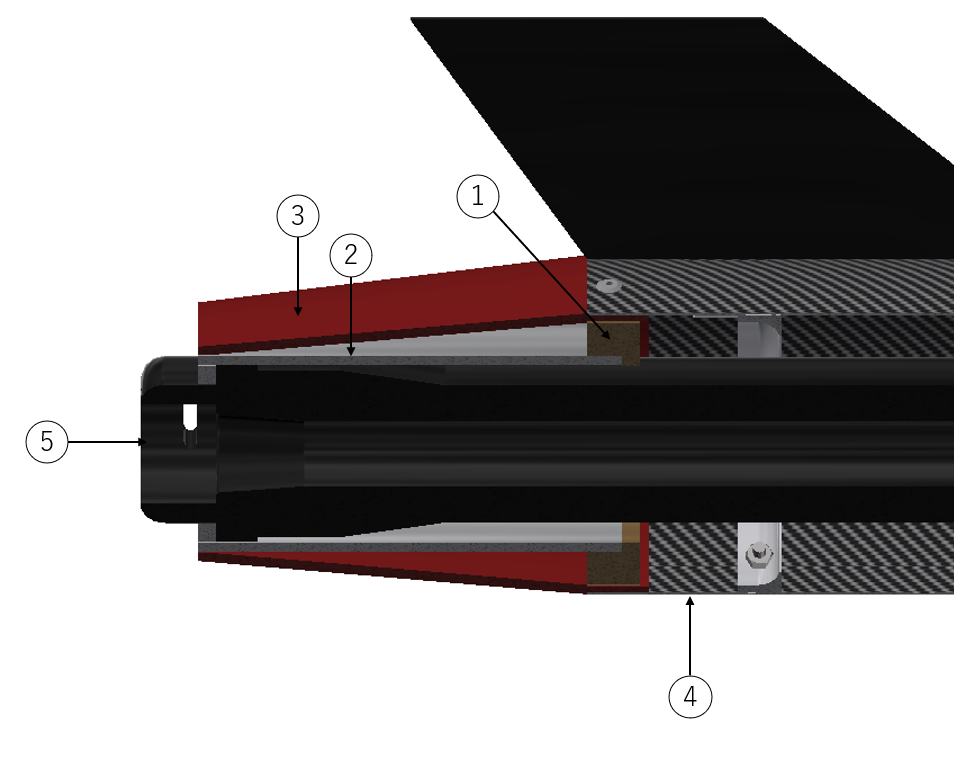
\includegraphics[scale = 0.4]{pic_str/s_talecorn_num.png}
    \caption{テールコーン付近断面図}
    \label{s_tale_num}
\end{figure}

\begin{table}[H]
    \centering
    \caption{テールコーン部品表}
    \begin{tabular}{ccc} \toprule
        No.&名称&材質、型番\\ \midrule
        1&エンジン受け1&A5052\\
        2&エンジン受け2&A5052\\
        3&テールコーン&ABS\\
        4&エンジンチューブ&CFRP\\
        5&エンジン&HyperTEK J250\\ \bottomrule
    \end{tabular}
    \label{s_tale_table}
\end{table}

\begin{figure}[H]
    \centering
    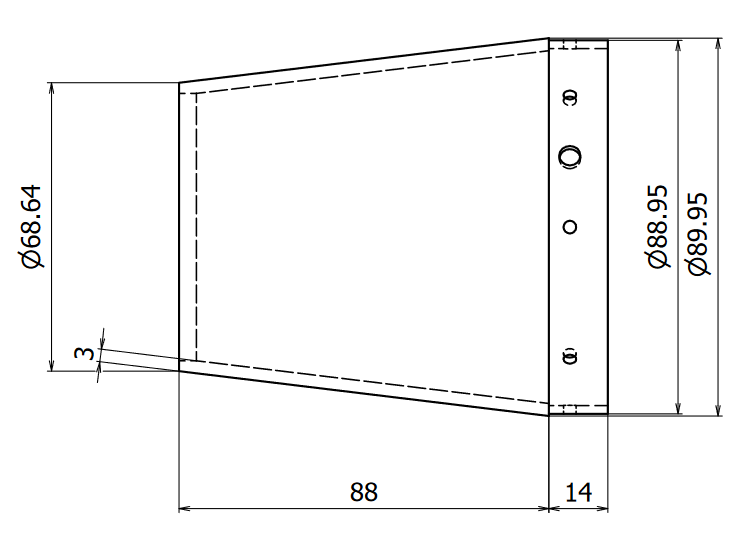
\includegraphics[scale = 0.6]{pic_str/s_talecorn_zumen.png}
    \caption{テールコーン図面}
    \label{s_tale_zumen}
\end{figure}

テールコーンを使用した際の効果については\red{どこか}に記す。
\blue{以下ではテールコーンについて特記点を記す。}
\begin{itemize}
    \item \blue{組立が困難である}\\
    図\ref{s_tale_num}に示すように、本設計ではエンジン受け1、2、テールコーン、エンジンチューブを一つのネジで止め構造になっている。
    組立の際に4部品全ての位相が合わない等の不具合が起きた。
    本番時はこれらの部品は全て組み立てた状態で輸送した。
    
    \item \blue{エンジンに近いため、テールコーンが一部燃えた}\\
    図\ref{s_tale_after1}、図\ref{s_tale_after2}に回収時のテールコーンの様子を示す。
    ここでは、落下時の強い衝撃によってABS製のテールコーンが一部破壊されたことが分かる。
    また、エンジンに近い部分が微小部分燃えていることが分かる。
    \red{~~~}
    
    \begin{figure}[H]
        \begin{tabular}{cc}
        \begin{minipage}[t]{0.45\hsize}
        \centering
        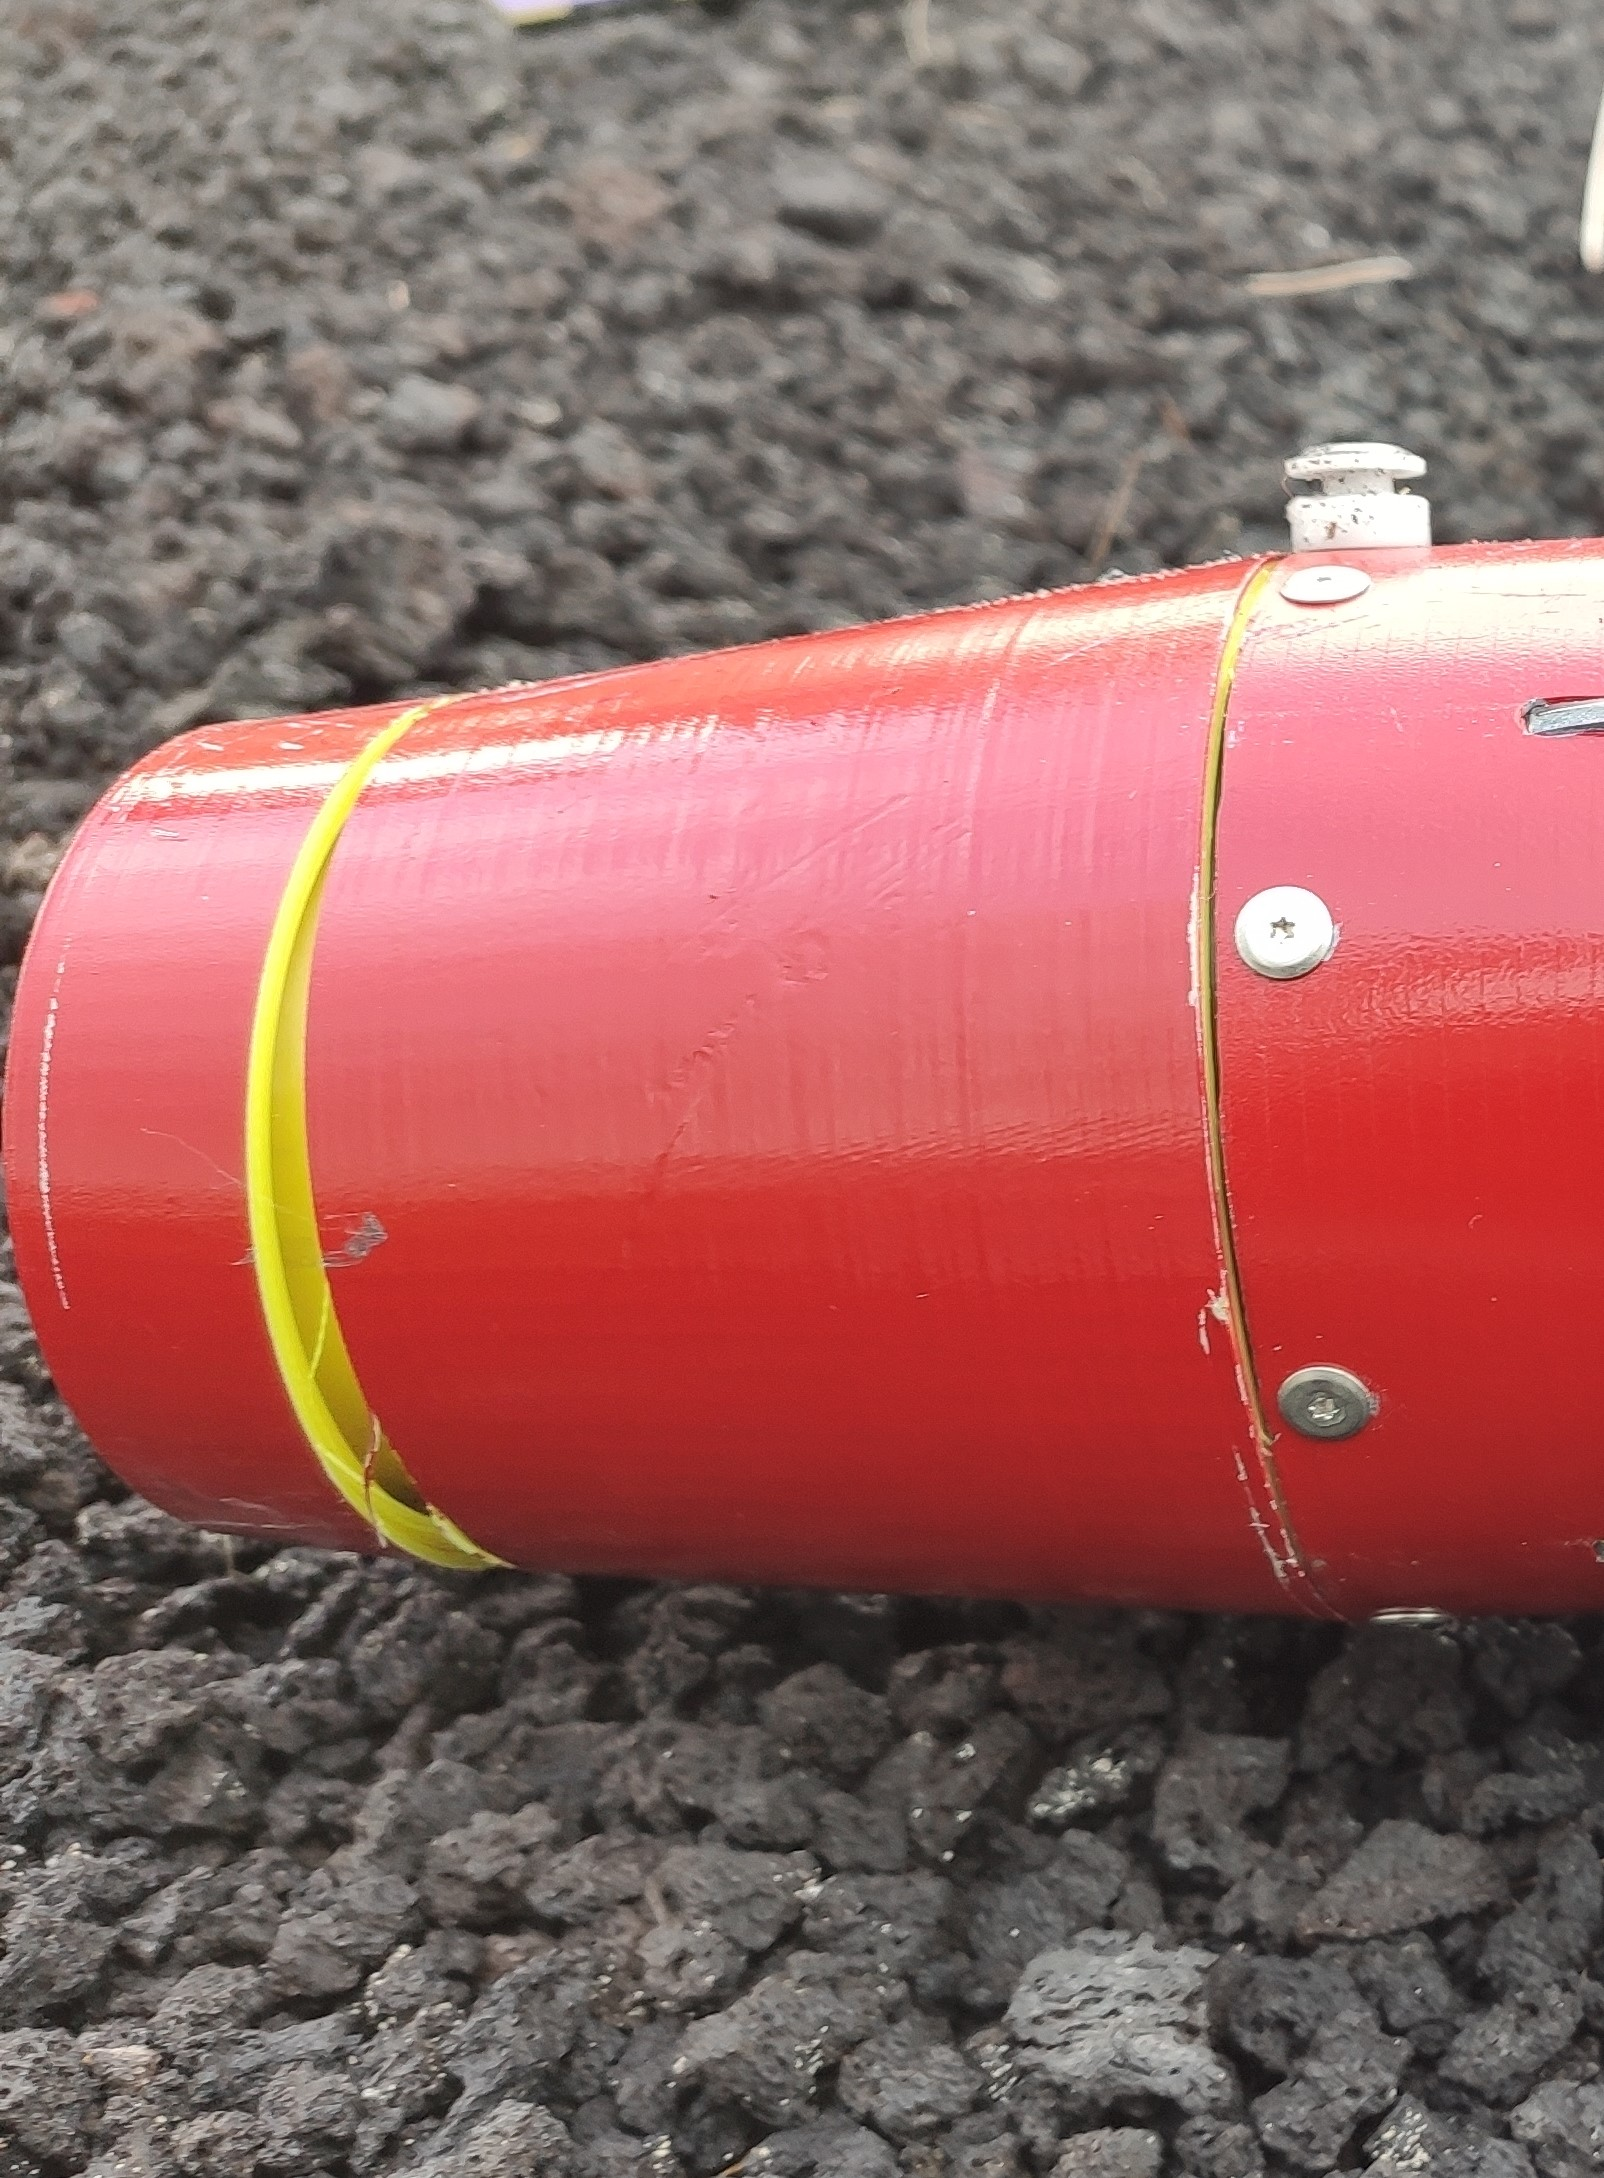
\includegraphics[scale = 0.1]{pic_str/s_tale_after2.jpg}
        \caption{テールコーン回収時様子}\label{s_tale_after1}
        \end{minipage}&
        \begin{minipage}[t]{0.45\hsize}
        \centering
        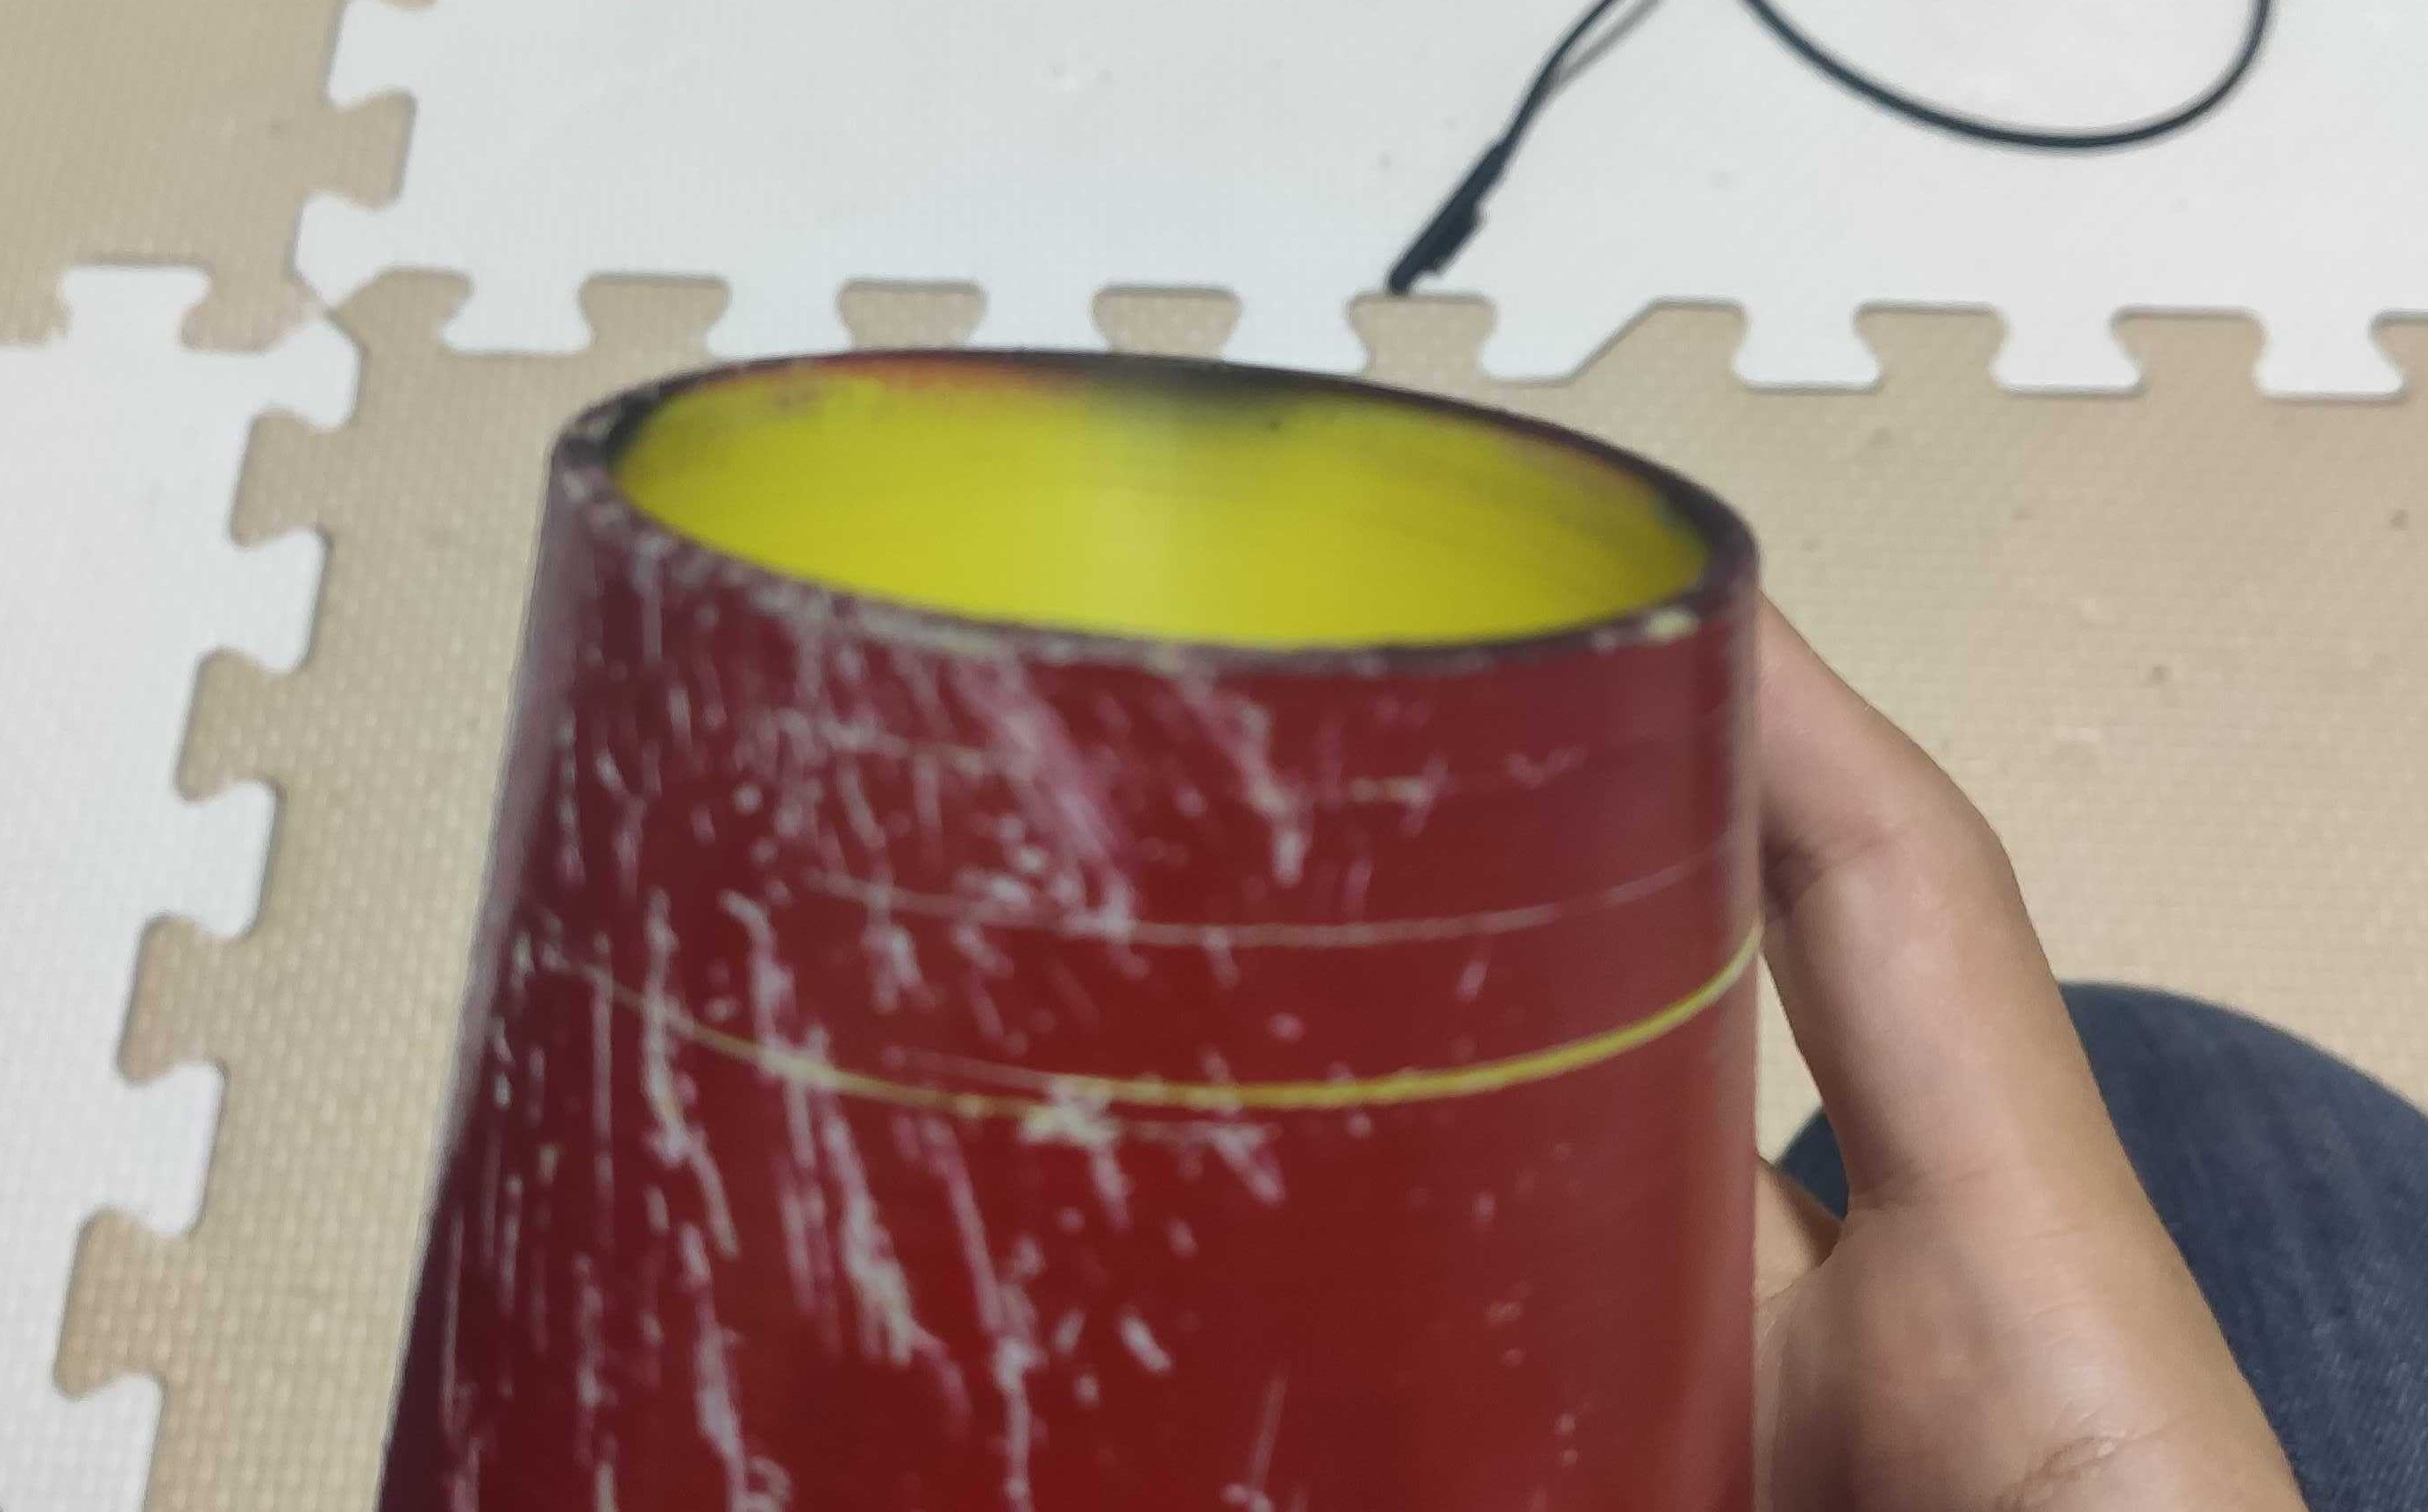
\includegraphics[scale = 0.1]{pic_str/s_tale_after1.jpg}
        \caption{テールコーン回収後様子}\label{s_tale_after2}
        \end{minipage}\end{tabular}
    \end{figure}
\end{itemize}

\red{結論。今後続けていくことはあるのか等。}

\subsection{打上結果}
\subsubsection{機体組立}
本打上実験ではウィンドウの順番が事前に決められておらず、現地審査合格状況とGSE展開状況で順番が決める事になっていたため、現地ではできるだけ短時間で組立られるような工夫をした。
具体的にはエンジン部はフィン含め完全に組み立てる、電装タワーも組み立てて行き当日一部配線のみを繋ぐ、組立練習を複数回行う等を行った。

打上実験1日目は、8:10頃打上実験本部に到着後すぐ組立を開始し、予定より10分ほど遅れて9:00頃に機体が完成した。
その後現地審査担当の到着と他機体の現地審査を待ち、9:45頃に本機体の現地審査を開始した。
現地審査では、完成報告書と最終審査書に不備があることが発覚し、その場でシミュレーションを行った上で問題が無いことを確認し、10:45頃に現地審査の合格した。
その後、11:40頃本部から射点に向けて機体を搬入した。
CRETAE1が13:00X、CREATE2(本機)が14:00Xの予定であったが、CREATE1打上げの際のGSEトラブルの影響で実験1日目の打上げは断念し、翌日に打ち上げることとした。

打上実験2日目は、午前2:20宿出発、2:40裏砂漠駐車場着、3:10裏砂漠駐車場発、3:45本部到着、という\blue{\sout{世紀末}}スケジュールで動き、風と気温の様子を見て4:20頃に組立を開始した。
2日目はおおよそ順調に進み、5:20には現地審査合格、6:00には射点に機体搬入完了した。
7:20頃からランチャー挿入、ステム挿入、ランチャー立上げ、総員退避が行われ、\blue{\sout{航空申請外の}}7:47に打上げられた。


\subsubsection{機体回収}
打上げは正常に点火し、離床後10.2秒後にパラシュートの開傘に成功した。

着地状況を図\ref{s_tyakuti_pic}に示す。
\begin{figure}[H]
    \centering
    \includegraphics[scale = 0.08]{pic_str/s_tyakuti_pic.jpg}
    \caption{着地状況}
    \label{s_tyakuti_pic}
\end{figure}

落下の衝撃でアクリル製の固定フィンと可動フィンが機体から外れ、機体の周りに散らばっている様子が確認できた。
また、cfrp製のノーズコーンも落下の衝撃で割れていることが確認でき、チューブの塗装が一部めくれ傷がついていた。
しかし、それ以外の搭載計器やエンジン、動翼機構には問題無いことをその後確認した。

\subsubsection{\blue{破損状況}}
本項では機体の破損状況とその原因について記す。
\begin{itemize}
    \item 固定フィン\\
    図\ref{s_tyakuti_pic}に示すように固定フィンは4枚とも機体から外れ、機体の周りに散らばっていた。
    これは落下の衝撃が原因であると考えられる。
    フィンはアクリル製のため、他部品と比べて折れやすいが、\red{~~~~}という理由でこれからも製作方式の変更は考えていない。
    \\
    \item 可動フィン\\
    設置した2枚の可動フィンのうち、1枚は機体のすぐ周りに落ちていたのが確認できたが、1枚は発見できなかった。
    原因として、パラシュート開放時に機体と分離したフェアリングが、動翼にあたって取れたことが考えられる。
    内部から撮影したカメラ映像のうち、、、、をそれぞれ図\red{???}に示す。
    以上より、パラシュート開放後に、フェアリングのようなものと防犯ブザーのようなものが確認でき、そのすぐ後に可動フィンが外れてなくなっていることが分かる。
    後日確認したが、フェアリングち機体を結ぶワイヤーは、動翼が届くのに十分な距離であった。(図\ref{s_fear}参照。)
    今後の機体に動翼を設置するときは、ワイヤーの長さを短くする等の対応が必要となる。
    
    \begin{figure}[H]
        \centering
        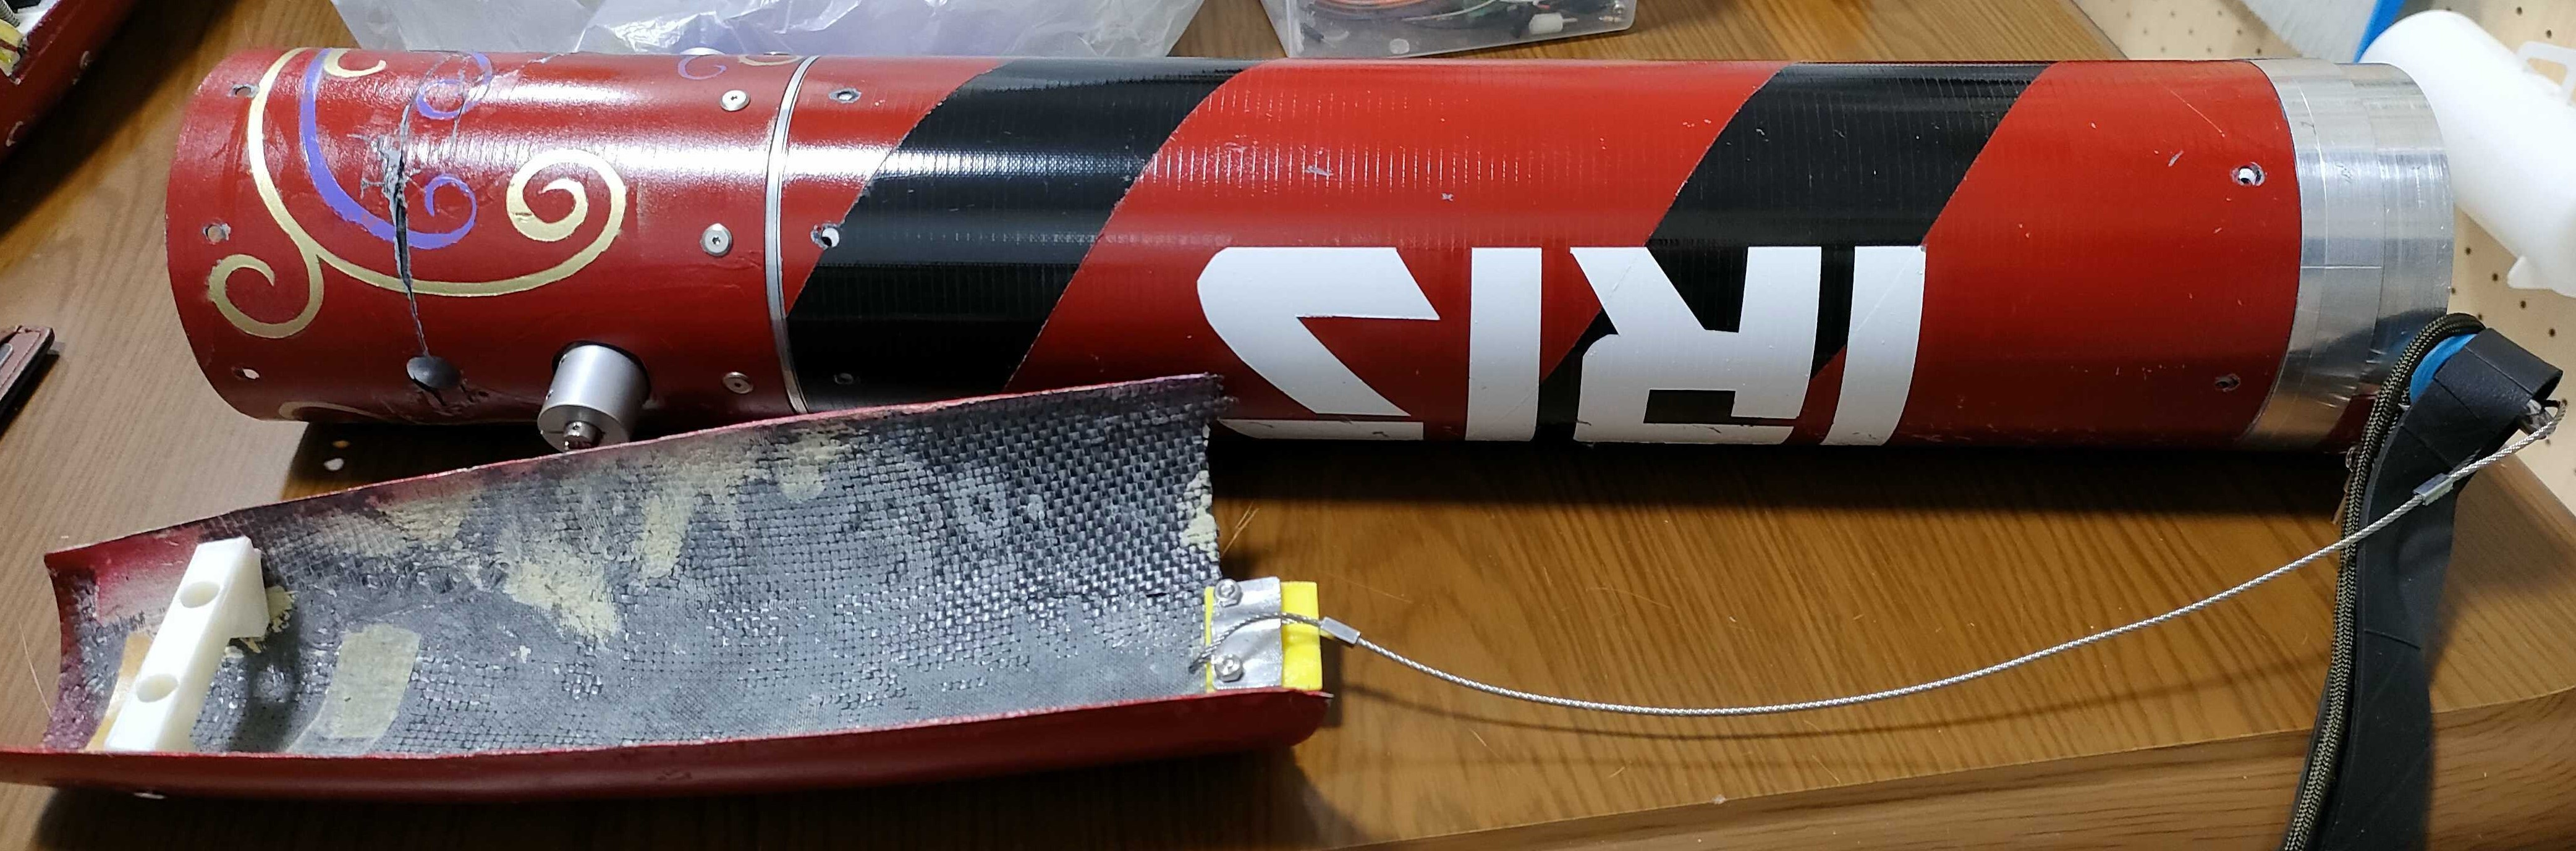
\includegraphics[scale = 0.12]{pic_str/s_fearring.jpg}
        \caption{フェアリングと可動フィンの位置関係}
        \label{s_fear}
    \end{figure}
    
    \item ノーズコーン及びピトー管\\
    機体回収時のノーズコーンの様子を図\ref{s_noze}に示す。
    図\ref{s_noze}より、ノーズコーンの根本付近から破断していることが確認できる。

    \red{原因?普通に着地の衝撃?エンジンから落ちるけど別に関係無いよね}
    \begin{figure}[H]
        \centering
        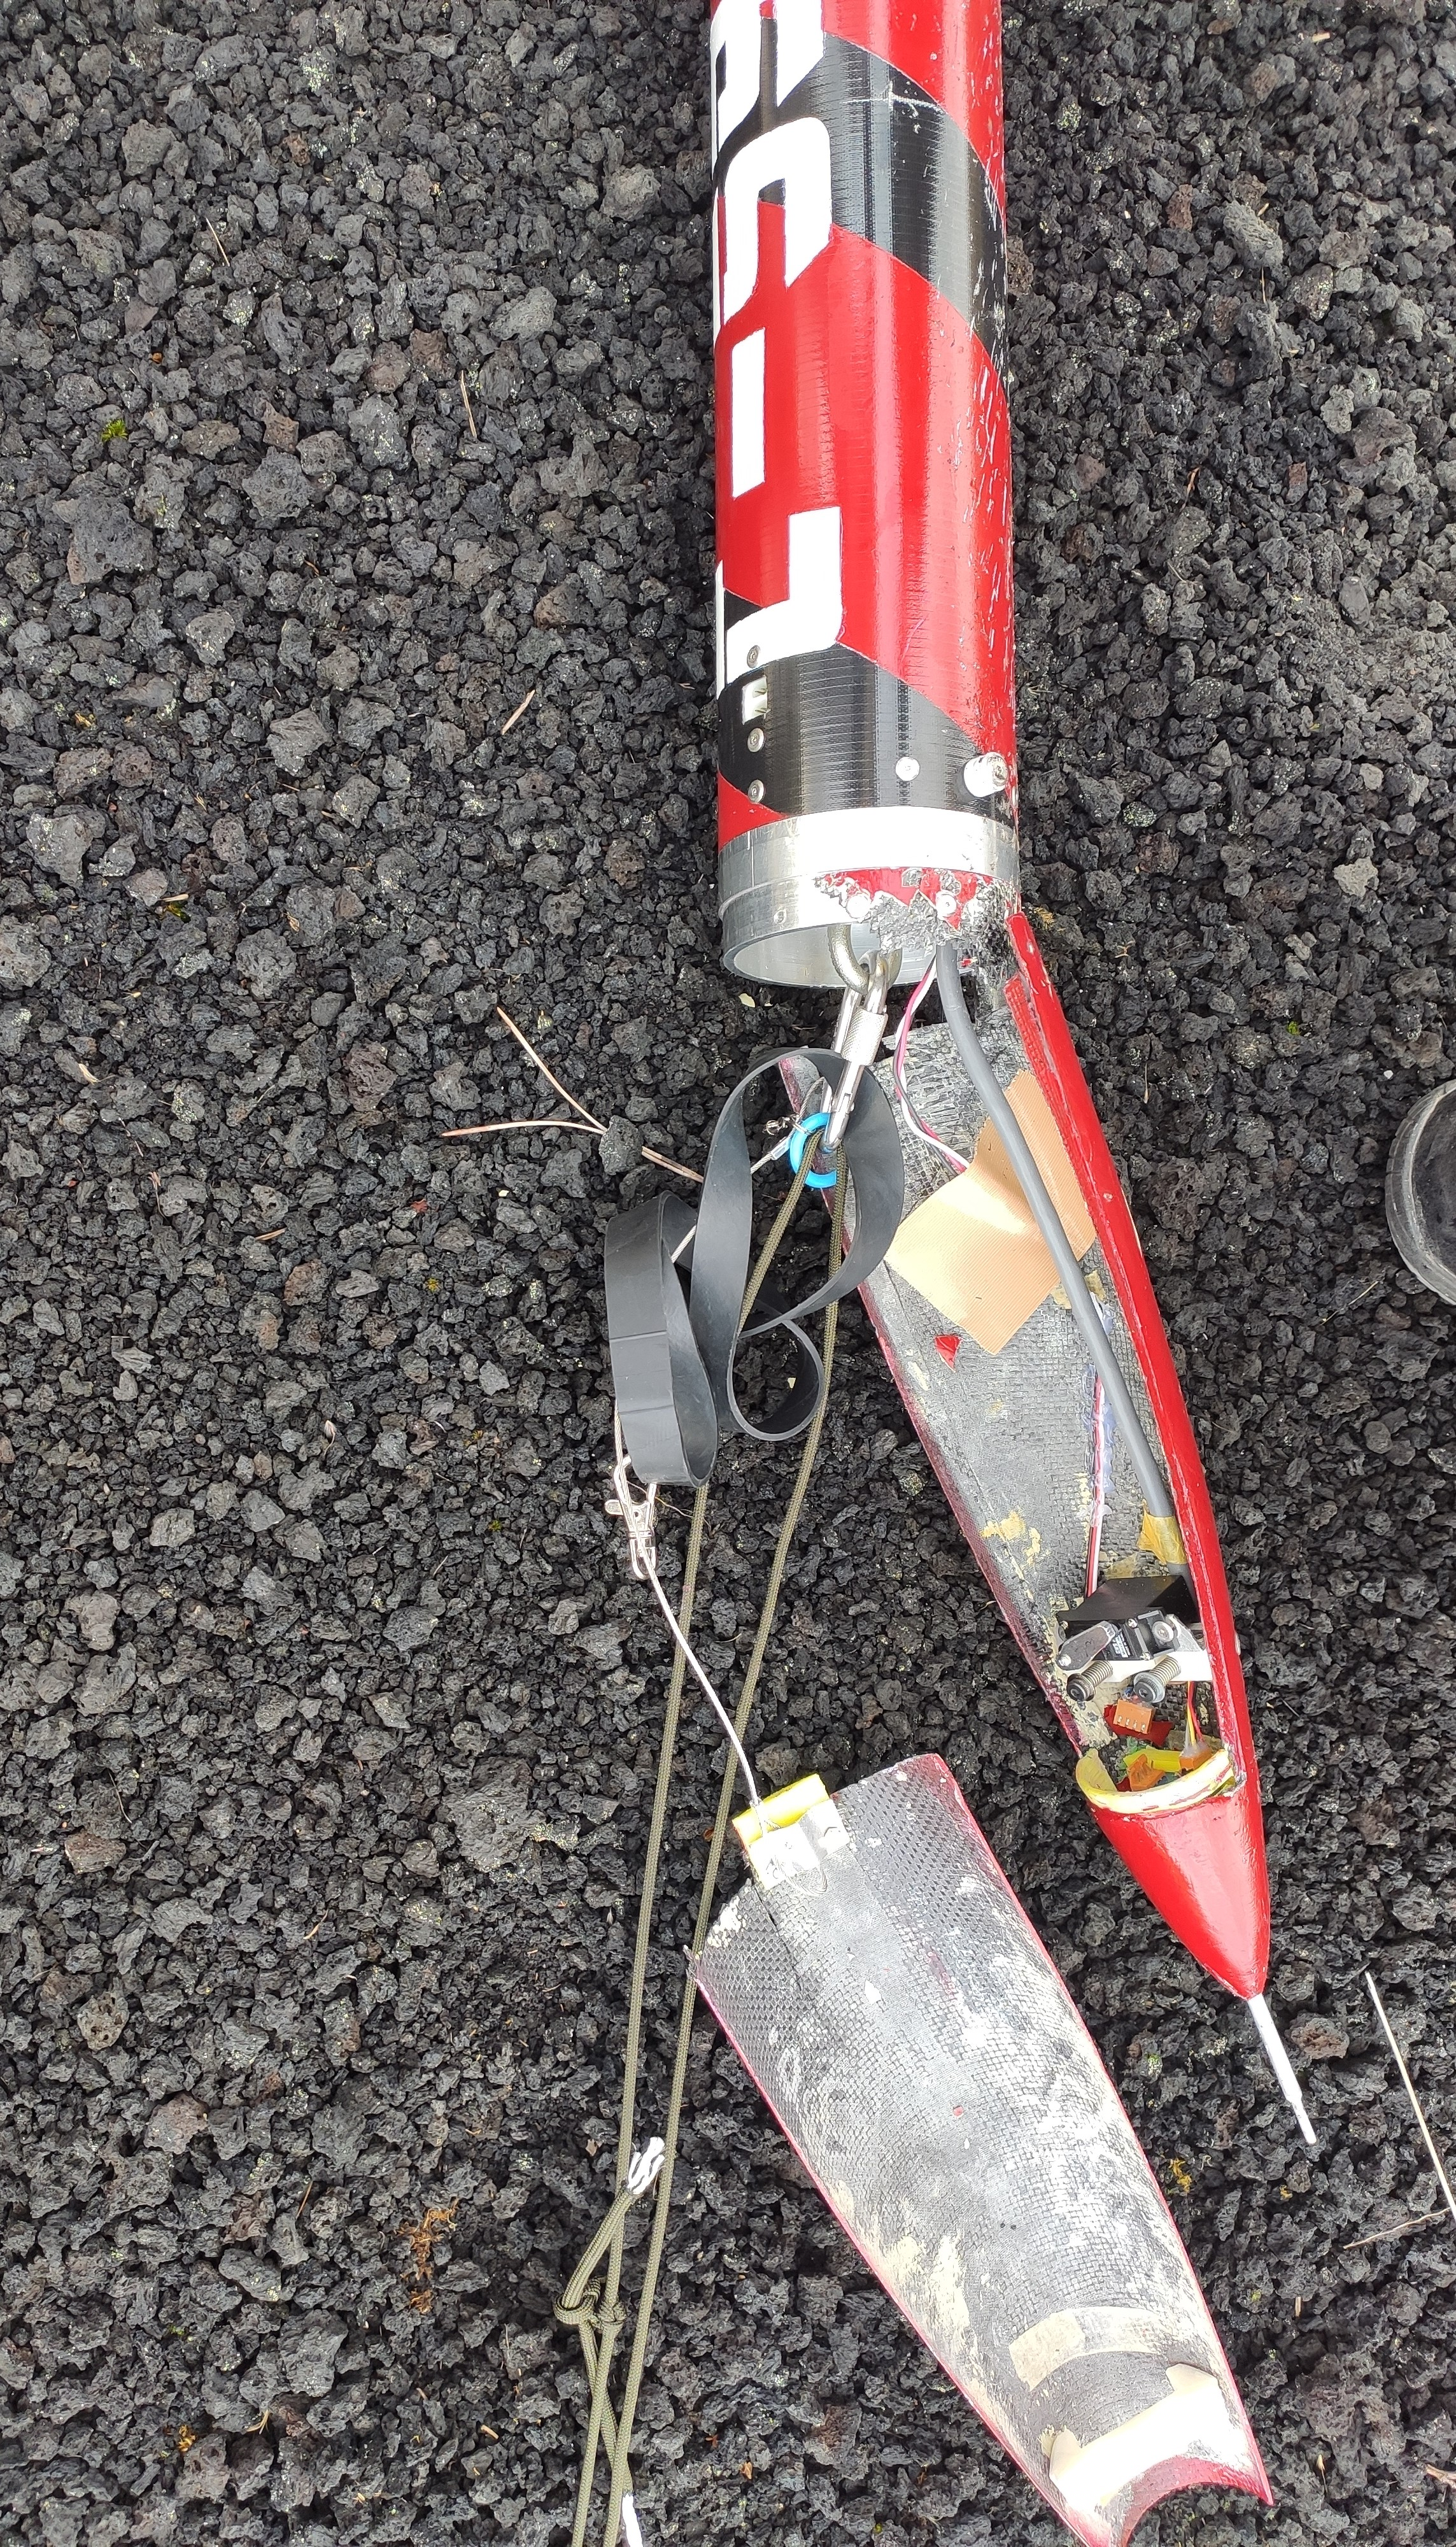
\includegraphics[scale = 0.1,angle = 270]{pic_str/s_tyakuti_noze.jpg}
        \caption{機体回収時のノーズコーン}
        \label{s_noze}
    \end{figure}

    また、同様に機体回収時のピトー管の様子を図\ref{s_tyakuti_pito}
    \footnote{ピトー管につながるケーブルが抜けているが、これは\red{~~~}のため発見後すぐにケーブルを抜いためであり、落下の衝撃で外れたわけではない。}、図\ref{s_tyakuti_pito2}に示す。

    ピトー管固定具(ABS製)はメタロックでノーズコーン(cfrp製)と固定されている。
    図\ref{s_tyakuti_pito2}から確認されているようにメタロックで固定されていない部分のピトー管固定具が破壊されていた。
    ピトー管にかなり強い力がかかったと思われる。\red{←なんかもっと}
    
    \begin{figure}[H]
        \begin{tabular}{cc}
        \begin{minipage}[t]{0.45\hsize}
        \centering
        \includegraphics[scale = 0.05]{pic_str/s_tyakuti_pito.jpg}
        \caption{機体回収時のピトー管[1]}\label{s_tyakuti_pito}
        \end{minipage}&
        \begin{minipage}[t]{0.45\hsize}
        \centering
        \includegraphics[scale = 0.05]{pic_str/s_tyakuti_pito_2.jpg}
        \caption{機体回収時のピトー管[2]}\label{s_tyakuti_pito2}
        \end{minipage}\end{tabular}
    \end{figure}
    
    \item 防犯ブザー\\
    CREATEでは、開傘衝撃を和らげ、パラシュートが開くと防犯ブザーが鳴り落下位置を知らせる機構の、通称「ショックアブソーバ」を取り付けている。
    今回、ショックアブソーバについている防犯ブザーが紛失した。図\red{?}に写っているように、防犯ブザーはパラシュート開傘時に外れたと考えられる。
    
    ショックアブソーバの機構図を図\red{??}に示す。
    今回は、開傘時に図\red{??}に示した赤丸の部分が破壊され、防犯ブザーのピンが抜けている状態で機体が発見されたので、防犯ブザーが分離されてしまいロストしてしまった。
    実際に機体から撮影した映像には、防犯ブザーが外れ飛んでいく様子が確認できる。

    分析の結果、防犯ブザーの\red{~~}の部分が脆弱なことが分かったため、次回以降の機体ではこの部分を補強することとした。

    \red{もう少し具体的に書こうかな}
    \\
    \item カメラ\\
    飛翔中に可動フィンが実際に動いていること、ロール制御することでロール方向に回転しない映像を撮ることを目的に、機体内にカメラを配置した。
    このカメラはABS製のカメラ固定治具でカメラと錘を固定したが、着地時の衝撃によりカメラ固定治具が破損していた。
    その様子を図\ref{s_tyakuti_camera}に示す。\red{2ko 1ko}
    \begin{figure}[H]
        \centering
        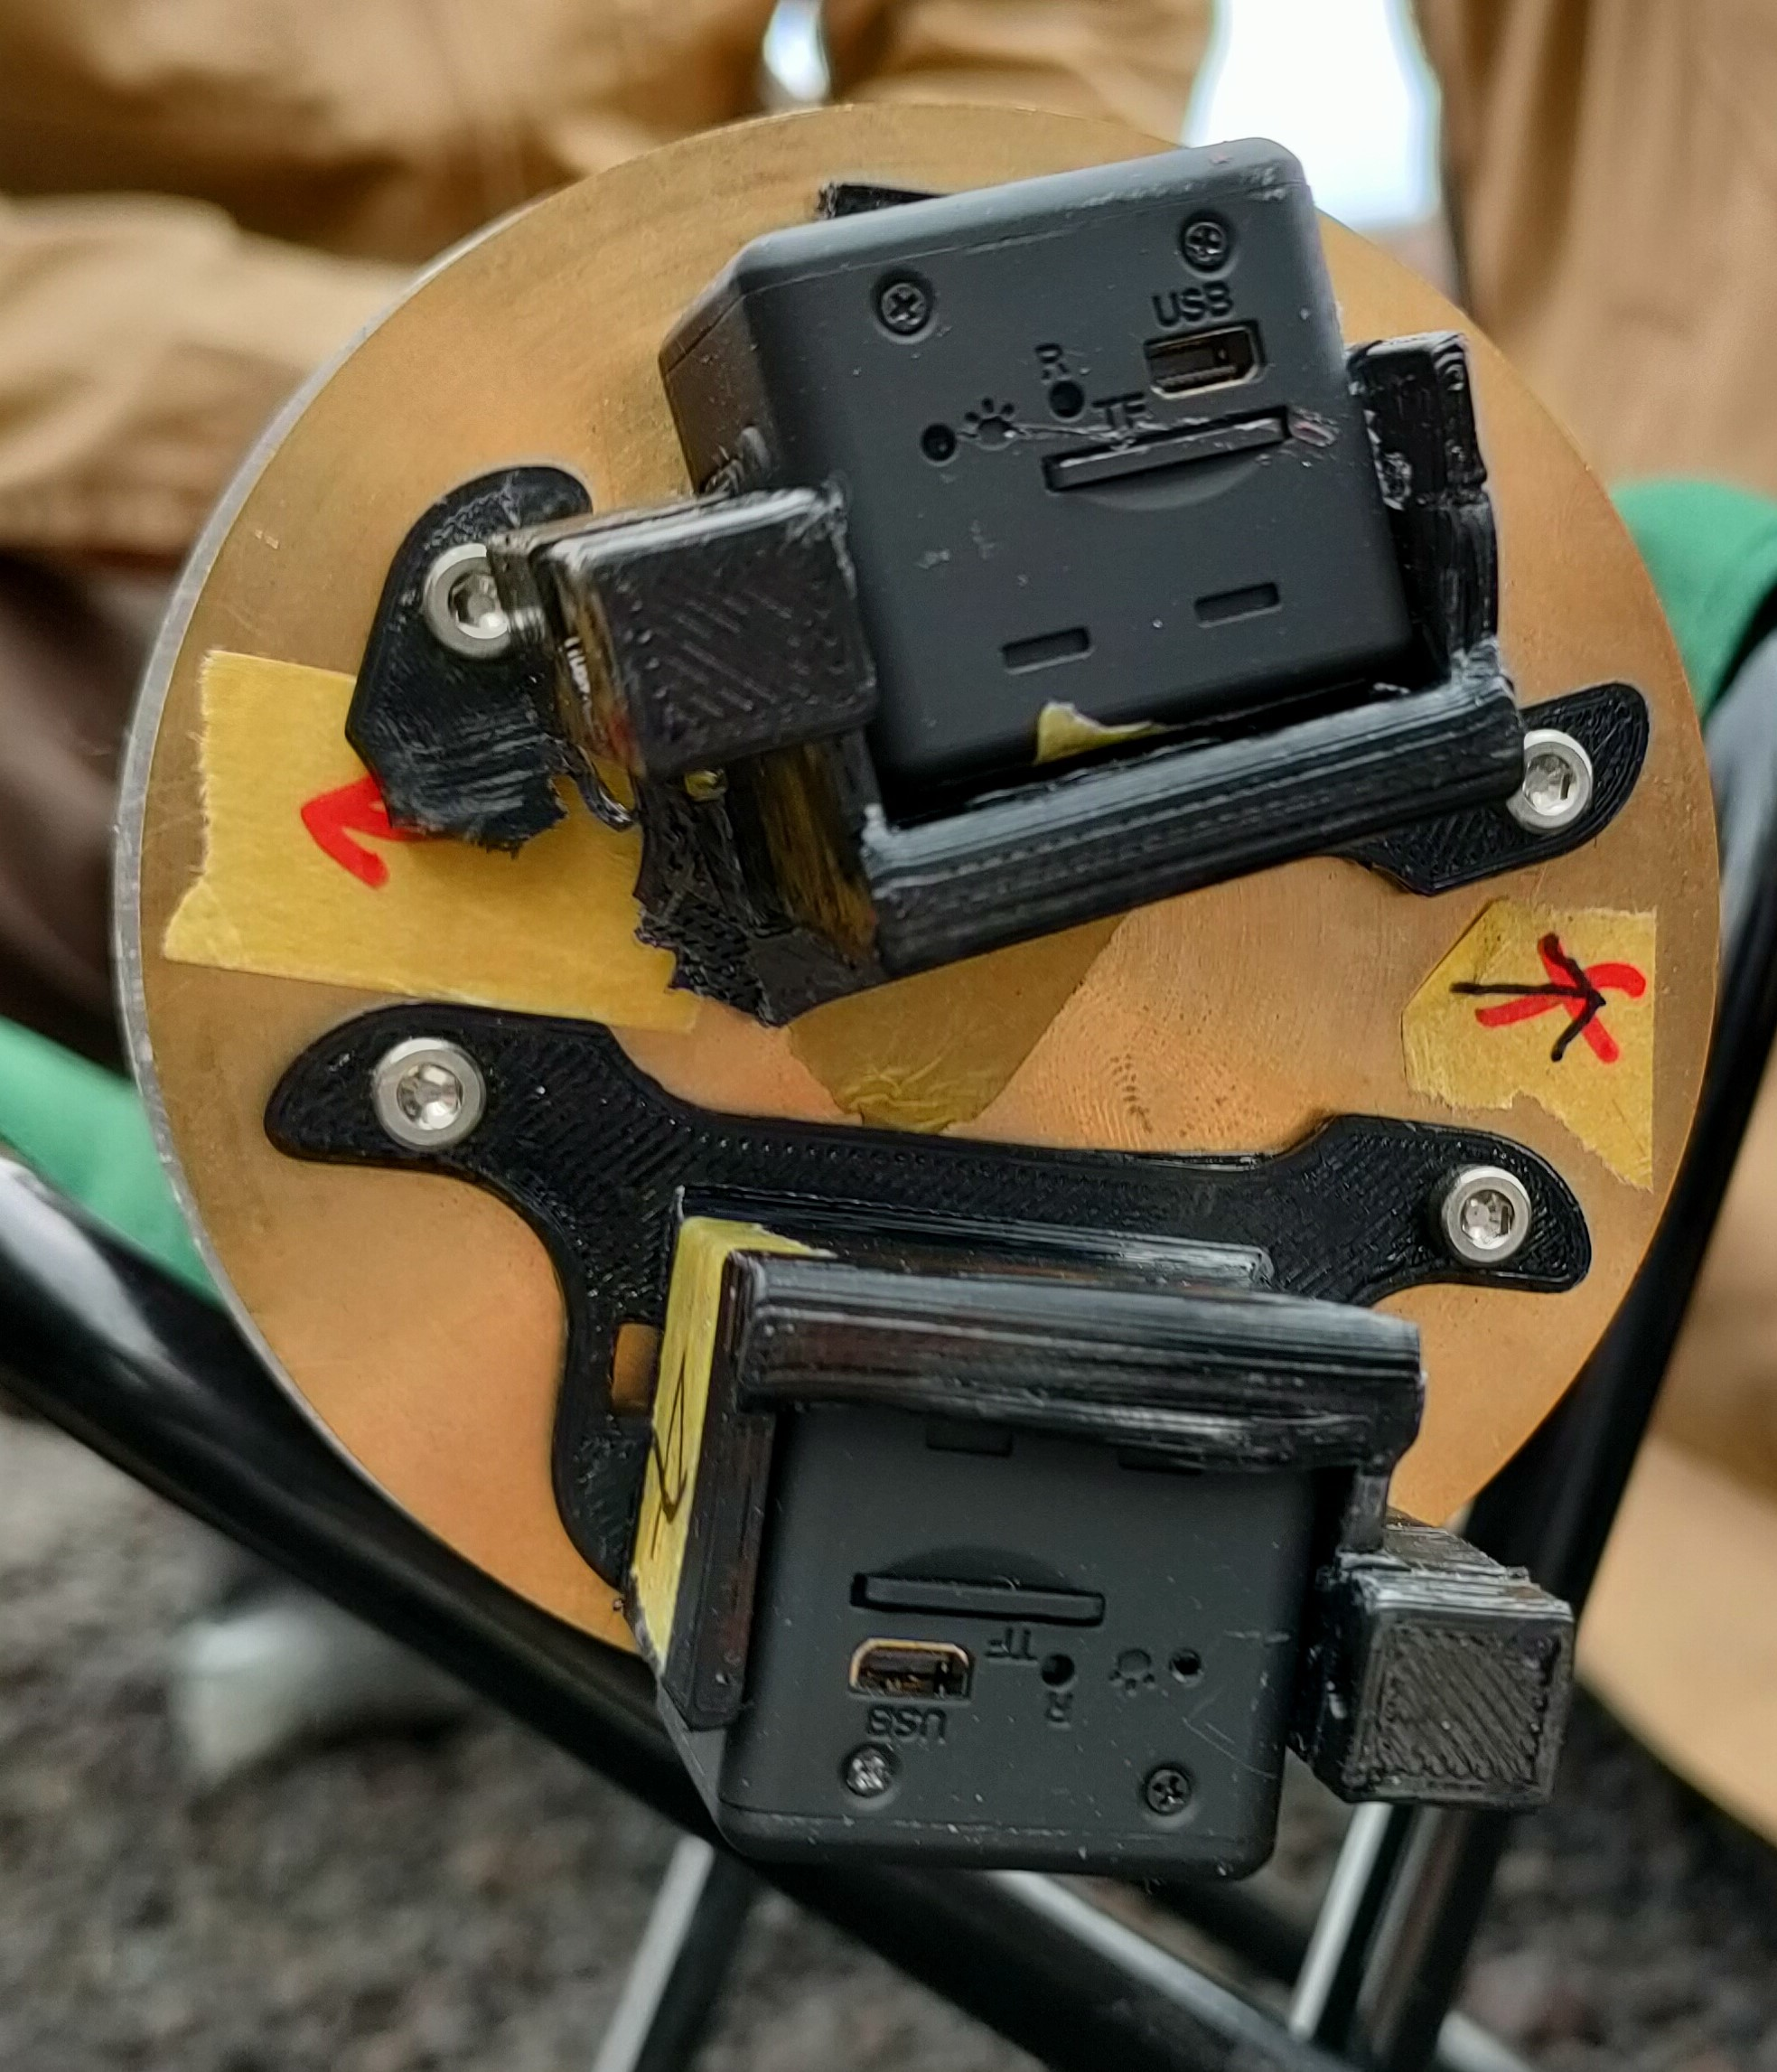
\includegraphics[scale = 0.1]{pic_str/s_tyakuti_camera.jpg}
        \caption{機体回収時のカメラの様子}
        \label{s_tyakuti_camera}
    \end{figure}
    本カメラは今回の機体独自のものであり、仮に開傘時の衝撃や着地時の衝撃で破損しても問題ないという想定のもとで設計したので、問題はないと考える。
    \\
    \item テールコーン\\
    図\ref{s_tale_after1}に示すように、着時時の衝撃でテールコーンの一部が破損した。
    \red{どうしよっかな}
    \\
    \item GPSモジュール\\
    GPSは図\ref{s_GPS_nodamage}のような形状をしているが、図\ref{s_GPS_damage}のように上部の部分が取れてしまっていた。
    着時時の衝撃ではがれたのだと考えられる。
    次回以降の機体では、GPSのモジュールの上部の部分はグルーガンで接着することとした。
    
    \begin{figure}[H]
        \begin{tabular}{cc}
        \begin{minipage}[t]{0.45\hsize}
        \centering
        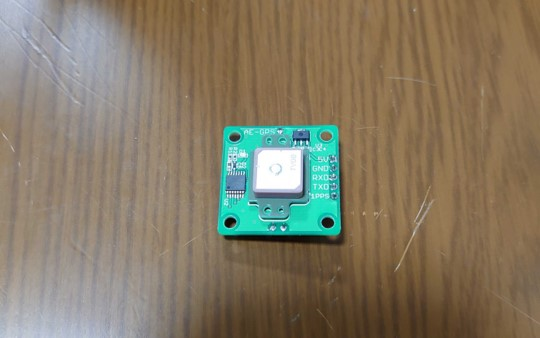
\includegraphics[width=0.8\linewidth]{pic_str/GPS_nodamage.jpg}
        \caption{GPSモジュール}\label{s_GPS_nodamage}
        \end{minipage}&
        \begin{minipage}[t]{0.45\hsize}
        \centering
        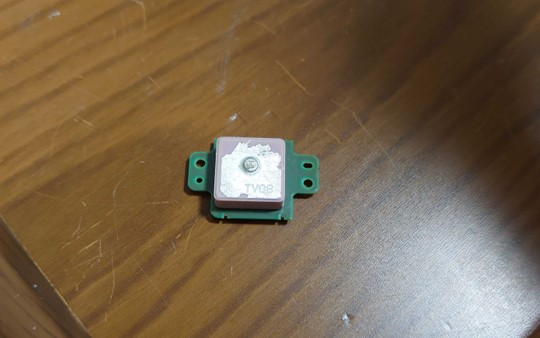
\includegraphics[width=0.8\linewidth]{pic_str/GPS_damage.jpg}
        \caption{GPSモジュールの破損の様子}\label{s_GPS_damage}
        \end{minipage}\end{tabular}
    \end{figure}
    
\end{itemize}


\end{document}